% \documentclass[journal=jacsat,manuscript=article,layout=twocolumn]{achemso}
\documentclass[5p,times]{elsarticle}

\usepackage[T1]{fontenc}       % Use modern font encodings


\usepackage{xcolor}
\usepackage{textcomp}
\usepackage{geometry}
\usepackage[normalem]{ulem}
\usepackage{amsmath}
\usepackage{amssymb}
\usepackage{graphicx}
\usepackage{lineno,hyperref}
\hypersetup{
    colorlinks=true,
%     linkcolor=cyan,
%     filecolor=magenta,      
%     urlcolor=cyan,
}
% \modulolinenumbers[5]

\newcommand*{\ga}{\alpha}
\newcommand*{\gb}{\beta}
\newcommand*{\gam}{\gamma}
\newcommand*{\gd}{\delta}
\newcommand*{\eps}{\epsilon}
\newcommand*{\veps}{\varepsilon}
\newcommand*{\gz}{\zeta}
\newcommand*{\gt}{\theta}
\newcommand*{\gi}{\iota}
\newcommand*{\gk}{\kappa}
\newcommand*{\gl}{\lambda}
\newcommand*{\gs}{\sigma}
\newcommand*{\go}{\omega}
\newcommand*{\Gam}{\Gamma}
\newcommand*{\gD}{\Delta}
\newcommand*{\gT}{\Theta}
\newcommand*{\gL}{\Lambda}
\newcommand*{\gS}{\Sigma}
\newcommand*{\gO}{\Omega}
\newcommand*{\pt}[1]{\left( #1\right)}
\newcommand*{\pq}[1]{\left[ #1 \right]}
\newcommand*{\pg}[1]{\left\{ #1\right\}}
\newcommand*{\figref}[1]{\figurename~\ref{#1}}
\newcommand*{\red}[1]{\textcolor{red}{#1}}
\newcommand*{\blue}[1]{\textcolor{blue}{#1}}
% \newcommand*{\gray}[1]{\textcolor{gray}{#1}}
% \renewcommand{\baselinestretch}


%%%%%%%%%%%%%%%%%%%%%%%%%%%%%%%%%%%%%%%%%%%%%%%%%%%%%%%%%%%%%%%%%%%%%
%% Meta-data block
%% ---------------
%% Each author should be given as a separate \author command.
%%
%% Corresponding authors should have an e-mail given after the author
%% name as an \email command. Phone and fax numbers can be given
%% using \phone and \fax, respectively; this information is optional.
%%
%% The affiliation of authors is given after the authors; each
%% \affiliation command applies to all preceding authors not already
%% assigned an affiliation.
%%
%% The affiliation takes an option argument for the short name.  This
%% will typically be something like "University of Somewhere".
%%
%% The \altaffiliation macro should be used for new address, etc.
%% On the other hand, \alsoaffiliation is used on a per author basis
%% when authors are associated with multiple institutions.
%%%%%%%%%%%%%%%%%%%%%%%%%%%%%%%%%%%%%%%%%%%%%%%%%%%%%%%%%%%%%%%%%%%%%
 \journal{Journal of Theoretical Biology}
\bibliographystyle{elsarticle-num}



\begin{document}

\begin{frontmatter}

\title{How might random prebiotic polymers have become informational?}
% 
\author[addr1]{Elizaveta A. Guseva}
\ead{eguseva@tutanota.com}
\author[addr2]{Ronald N. Zuckermann}
\ead{rnzuckermann@lbl.gov }
\author[addr1]{Ken A. Dill\corref{mycorrespondingauthor}}
\cortext[mycorrespondingauthor]{Corresponding author}
\ead{dill@laufercenter.org}
% 
\address[addr1]{Laufer Center for Physical and Quantitative Biology, Stony Brook 
University, Stony Brook, NY, (United States)}
\address[addr2]{Lawrence Berkeley National Laboratory (LBNL), Berkeley, CA (United States)}

\begin{abstract}
We explore three questions of prebiotic chemistry:  
(1) Current prebiotic polymer syntheses produce mainly short chains.  How did longer chains -- 
which are thought to be needed to initiate the first stages of biology -- arise?  (2) How might 
random chain polymerizations have led to specific informational sequences?  (3) The 
Chemistry-to-Biology (CTB) transition is thought to require autocatalytic sets.  What molecular 
conformations might have been involved?  We use the HP lattice model of protein-like chains, which 
can explore sequence-structure 
relationships in an exhaustive and unbiased way.  We hypothesize that short random-sequence polymers 
of hydrophobic ($H$) and polar ($P$) monomers collapse into relatively compact structures, which 
exposes hydrophobic surfaces, acting as primitive versions of today's protein catalysts and 
elongating 
other such HP polymers.  We show that our mechanism leads to  autocatalytic 
dynamics of random HP chains; it produces populations that slowly increase in the overall degree 
of polymerization,  leading to domination of longer chains, and is sequence selective. 
Another feature of our model is its multimodality-capacity to settle at multiple distinct 
quasistable states characterized by different groups of dominating polymers.
We believe that this mechanism is relevant to the early origins of life.
\end{abstract}

% 
\begin{keyword}
xxx
\end{keyword}

\end{frontmatter}
%%%MAIN TEXT%%%%
% \linenumbers
\section{Introduction} 

 What prebiotic polymerization processes might have produced long chains of protein-like or 
nucleic-acid-like molecules~\cite{Joyce1987,Abel2005}?  Specifically: What polymerization processes 
are autocatalytic?  How could they have produced chains that are longer than are currently observed 
in model prebiotic experiments?  And, how could they have led from random to informational polymers 
during the Chemistry-to-Biology (CTB) transition?  Our questions here are about the physics, not 
about the chemistry of the monomers, polymers or synthesis conditions.  
 
 \subsection{The Chemistry-to-Biology transition has been postulated to entail an autocatalysis 
process}
 
 Early on, it was recognized by Eigen, Kaufmann, Dyson, Prigogine and others that the CTB transition 
requires autocatalysis, \emph{i.e.} some form of positive feedback or bootstrapping among molecules 
in some 
way~\cite{eigen1971selforganization,Eigen1977,Eigen1978,Dyson1985,Prigogine1989,Kauffman1986}.  
Autocatalysis is invoked as an answer to how small concentrations of some molecule could have become 
amplified, self-sustaining and stable.
 
 There has been much subsequent work, both theoretical and experimental.  We first review a few key 
theoretical results.  A class of theoretical models called GARD (Graded Autocatalysis Replication 
Domain)~\cite{segre1998graded,Segre2000,Markovitch2012} predicts that artificial autocatalytic 
chemico-kinetic networks can lead to self-replication, with a corresponding amplification of some 
chemicals over others (called compositional bias). System experience certain degree of inheritance 
and is capable of adaptive evolution.  GARD models are a subset of `metabolism-first' mechanisms, 
which envision that small-molecule chemical processes precede information transfer, and precede the 
origins of biopolymers.  Wu and Higgs~\cite{Wu2009} have developed a model of RNA chain-length 
autocatalysis.  Authors envision that some RNA chains have the capability to act as polymerase 
ribozymes, leading to autocatalytic elongation of other RNAs.  A similar model asserts that 
autocatalytic chain elongation arises from template-assisted ligation and random 
breakage~\cite{Tkachenko2014}.  All these models are focused on the `pre-informational' world before 
heteropolymers begin to encode biological sequence-structure relationships.  
 
 Another class of models describes a `post-informational' heteropolymer world, in which there is 
already some tendency of chains to evolve.  In one such model, it is assumed that polymers serve as 
their own templates because of the ability of certain heteropolymers to concentrate their own 
precursors~\cite{nowak2008prevolutionary,Ohtsuki2009,Chen2012,Derr2012}.  This model supposes an 
ability of molecules to recognize ``self'', but doesn't specify how.  In another such 
model~\cite{Walker2012}, chains can undergo sequence-independent template-directed replication.  
This model produces not only functional sequences from the pool of none-functional ones, but also 
effectively explores sequence space.  Both types of post-informational models predict that 
template-directed replication enhances diversity~\cite{Derr2012}.   These are abstract
models insofar as they do not postulate molecular structures that might explain the autocatalytic 
step. Nor do they address the heteropolymeric or informational aspects of the chains.
 
 In addition, there have been many experimental studies.  There has been work to create artificial 
autocatalytic sets in the laboratory~\cite{VonKiedrowski1986,Lincoln2009,Vaidya2012}. Such systems 
are designed so that pairs of molecules can catalyze each other (i.e. autocatalysis), leading to 
exponential growth.  For example, mixtures of RNA fragments are shown to self-assemble spontaneously 
into self-replicating ribozymes that can form catalytic networks that can compete with others.  One 
limitation, however, in applying such studies to prebiotic origins is that these are fragments taken 
from existing ribozymes, so they don't address the question of the origins from more primitive and 
random beginnings.
 
  Here, we describe a theoretical model that seeks to bridge from the pre- to post-informational 
world, a process we call the Chemistry-to-Biology transition.  We seek a physical basis for how 
short chains could have led to longer chains, for how random chains led to specific sequences, and 
for a structural basis and plausible kinetics for a possible prebiotic autocatalytic transition.
   
 \section{The `Flory Problem': polymerization processes produce mostly short chains}
 \label{sec:flory} 

Many experiments show that either amino acids or nucleotides can polymerize 
under prebiotic conditions without enzymes, but that they lead to mostly short 
chains~\cite{Shock1992,Martin1998,PAECHT-HOROWITZ1970,Leman2004a,Orgel2004}.  Leman et al. showed 
that carbonyl sulfide (COS), a simple volcanic gas, brings about the formation of oligo-peptides 
from amino acids under mild conditions in aqueous solution in minutes to hours. But the products are 
mainly dimers and trimers~\cite{Leman2004a}.  Other processes that increase yield of  
oligomers include: adsorption to clays~\cite{Rao1980,Lambert2008} or 
minerals~\cite{Bernal1949,Ferris1996}, evaporation of tidal 
pools~\cite{Nelson2001}, concentration in ice through eutectic melts~\cite{Kanavarioti2001},  
freezing~\cite{Bada2004} or temperature cycles. Still length of the oligmers stay short.  For 
example, mixtures of Gly and Gly$_2$ grow to about 
6-mers after 14 days~\cite{Rode1997,Rode1999} on the various mineral catalysts such 
as calcium montmorillonite, hectorite, silica or alumina; or in the experiments of Kanavarioti 
polymers of oligouridylates reach lengths up to 11 bases long, with an average length of 4 
\cite{Kanavarioti2001} after samples of 
phosphoimidazolide-activated uridine we frozen in the presence of metal ions in dilute solutions.  
 Similar results are found in other polymers: a prebiotically 
plausible mechanism produces oligomers having a combination of ester and amide bonds up to length 14 
containing up to 7 amide linkages~\cite{Forsythe2015}.  

Thus, it remains a mystery how prebiotic processes could have overcome what we call the ``Flory 
Problem'' -- i.e. the tendency of any polymerization process to produce more short chains and fewer 
long chains.  It is commonly assumed that the chain lengths of proteins or nucleic acids that could 
have initiated the transition to biology must be at least 30-60 monomers long~\cite{Szostak1993}.  
 
 Yet, since the earliest work of Flory and others, which elucidated basic polymerization mechanisms, 
it has been clear that long chains are \textit{exponentially} less populated than shorter chains.  
Standard 
processes of chain polymerization lead to the the Flory or Flory-Schulz distribution of the 
concentrations of chains of different chain 
lengths~\cite{Flory1953}. 
\begin{equation}
 f(a)=a^2l(1-a)^{l-1},\label{eq:flory}
\end{equation} 
where $l$ is the chain length and $a$ is the probability of chain termination, 
which is a measure of the average chain length: $\langle l \rangle = a(2- a)$.
Figure \ref{fig:flory}(a) shows the central prediction of Flory theory, that 
longer chains are exponentially less populated than shorter chains.  For example (see the magenta 
line 
in Fig~\ref{fig:flory}(a)):
\begin{equation}  
\frac{\pq{10~\mathrm{mers}}}{\pq{1~\mathrm{mers}}}\propto10^{-4},\qquad\frac{\pq{20~\mathrm{mers}}}
{
\pq{1~\mathrm{mers}}}\propto10^{-9}
\end{equation} 
Thus, for a synthetic process that starts with micromolar concentrations of monomers, the 
average chain length would be $\langle l \rangle = 2$ and 40-mers would have 
negligible concentrations of $\propto 10^{-19} $ mol/L. 
\begin{figure}[h!]
  \centering
  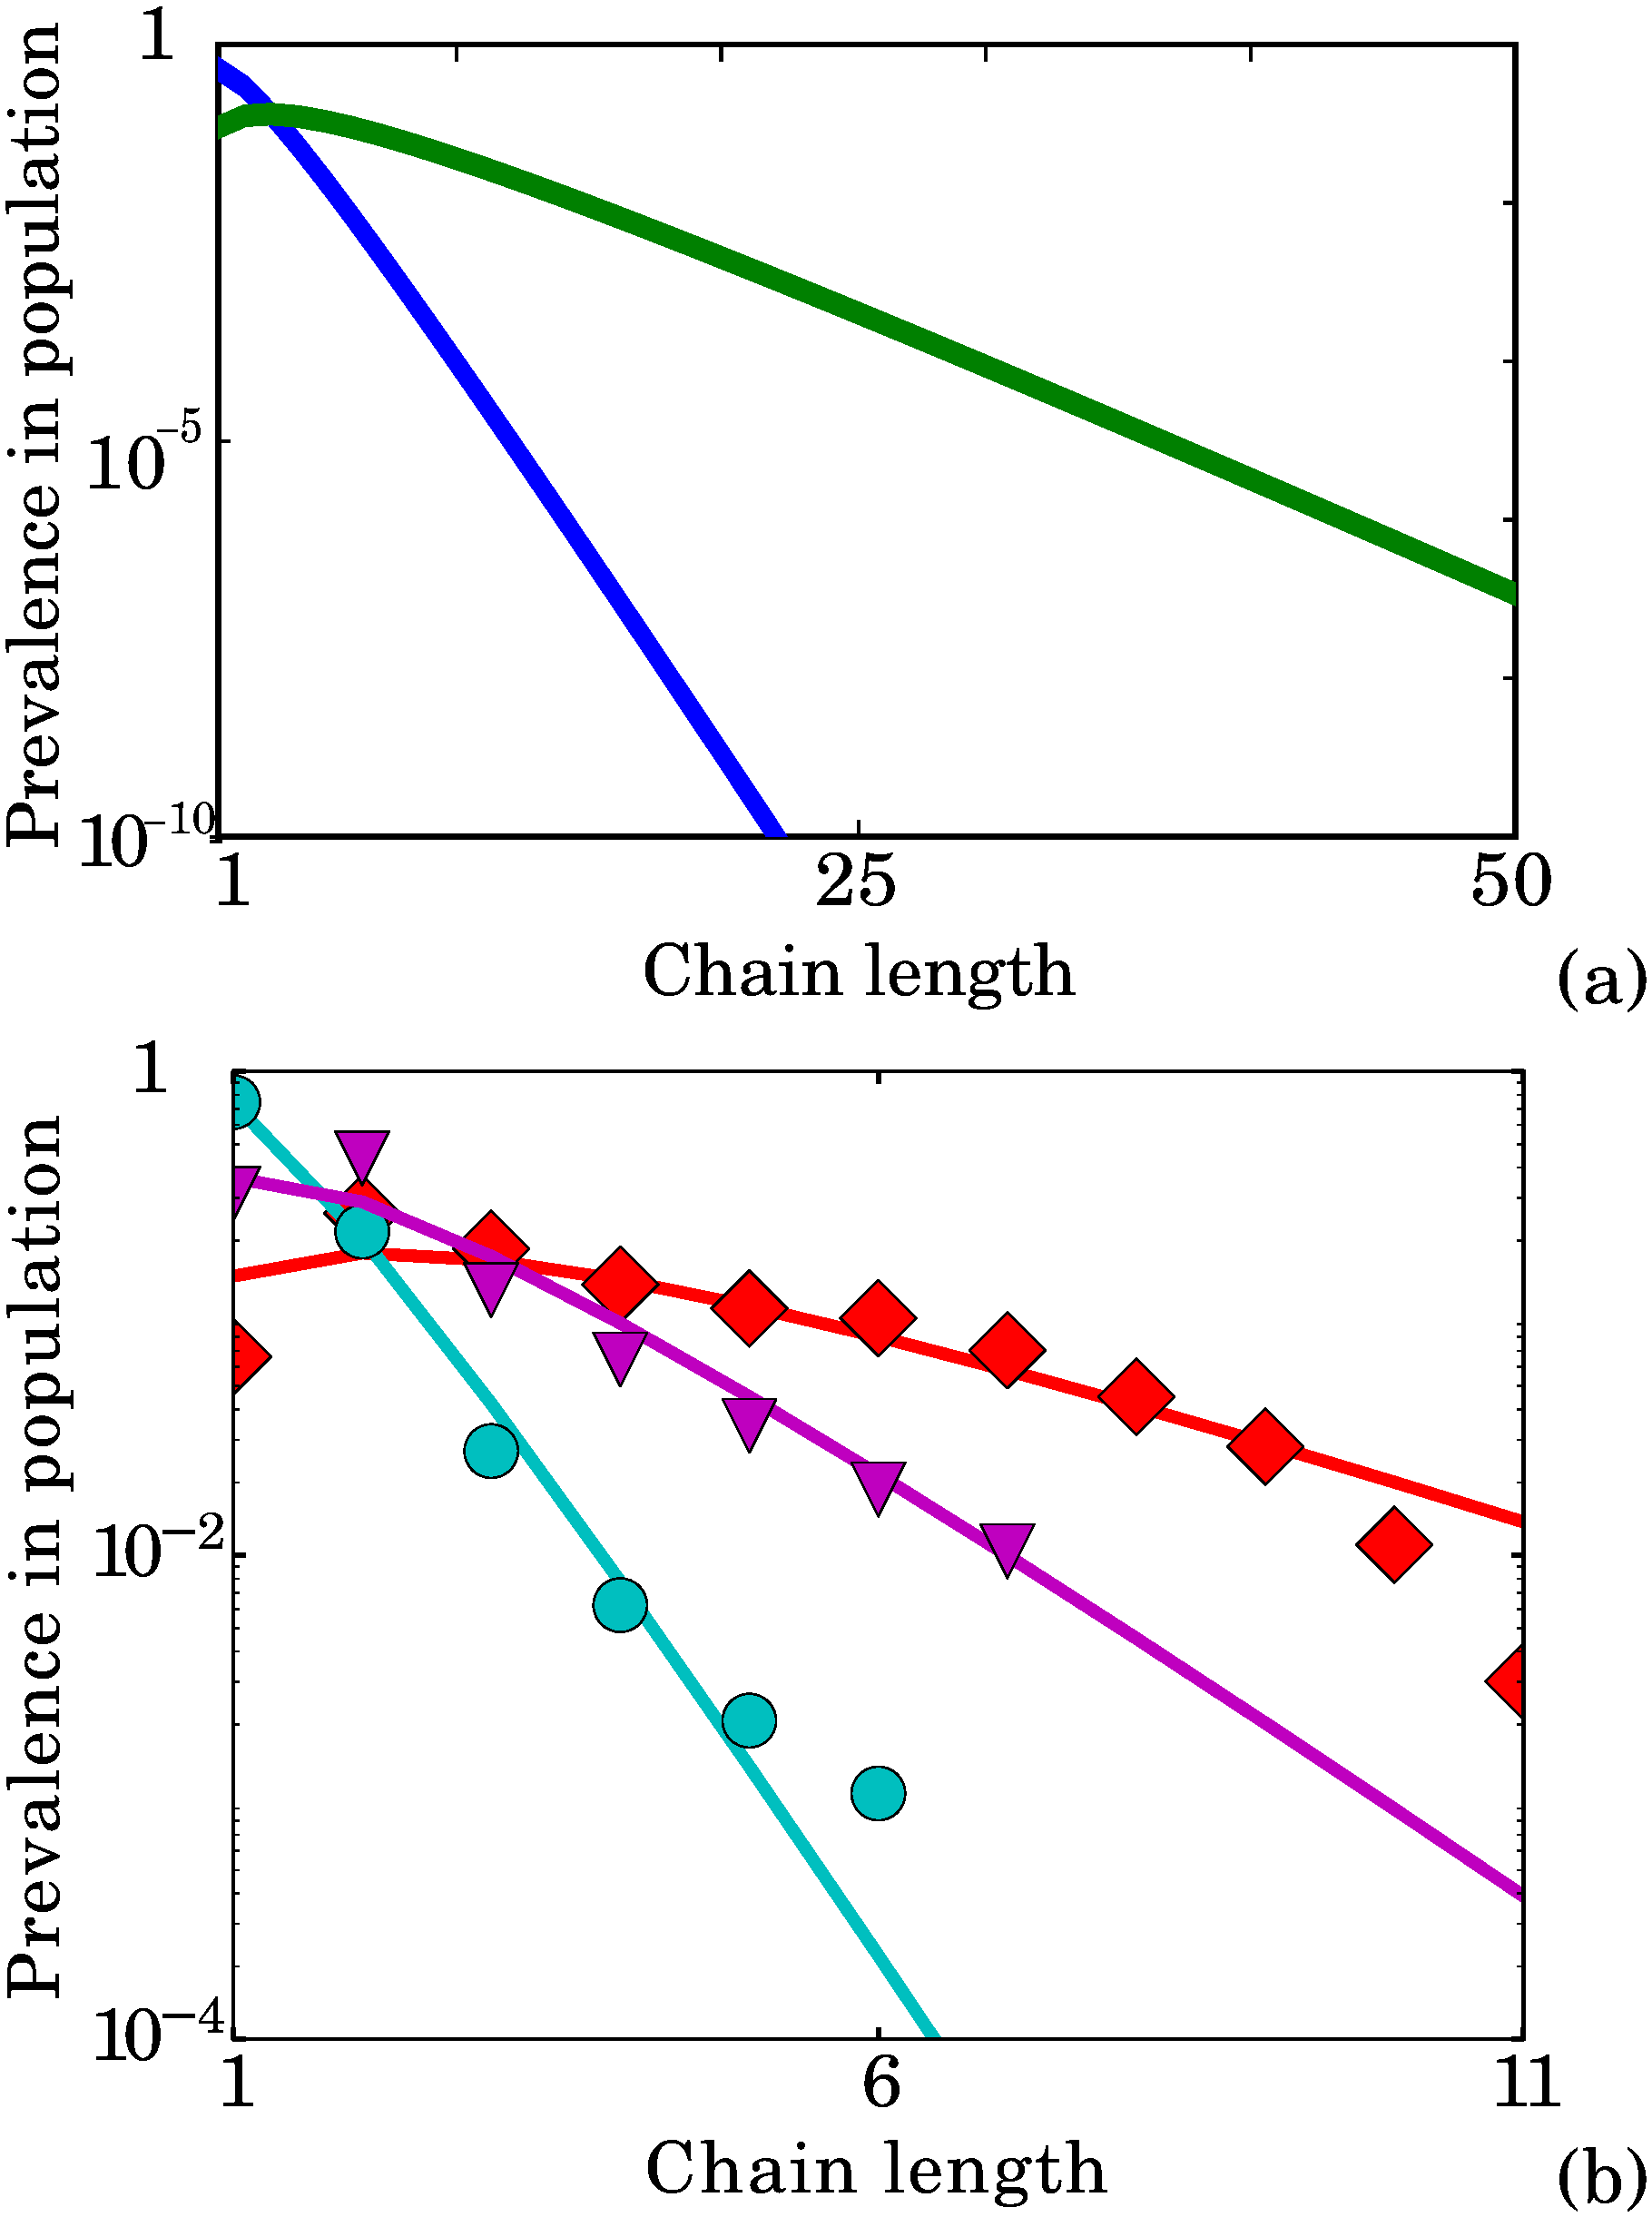
\includegraphics[width=0.9\columnwidth]{pictures/flory-two.pdf} \\
%  (b) 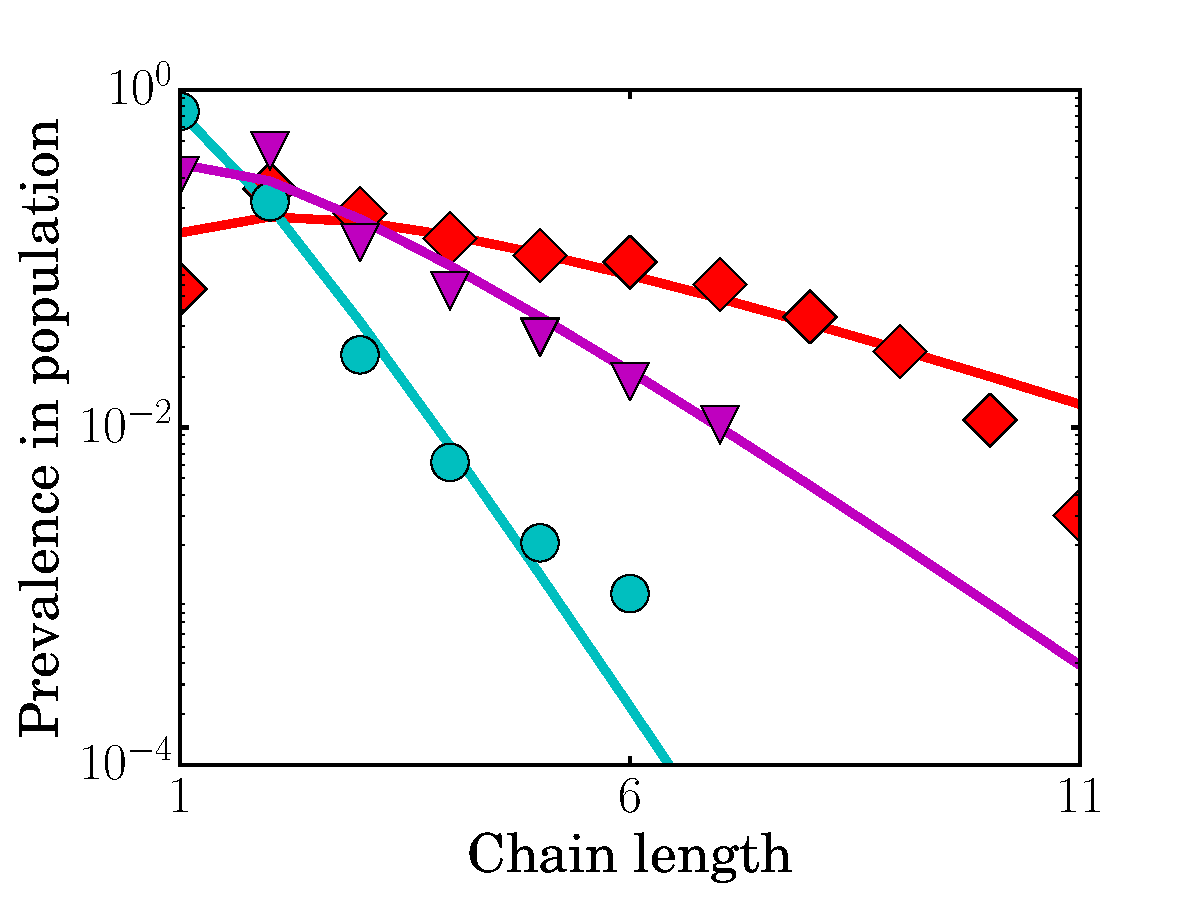
\includegraphics[width=0.9\columnwidth]{pictures/some_flory.pdf} 
  \caption{\textbf{Polymerization processes lead to mostly short chains.} (a)  Spontaneous 
polymerization processes typically lead to the Flory distribution of chain lengths. 
Green line gives $\langle  l \rangle= 6$, magenta one corresponds to $\langle l \rangle=2$
(b) Fitted distributions from experiments on prebiotic polymerization: red -- 
Kanavarioti~\cite{Kanavarioti2001}, cyan -- Ding~\cite{Ding1996}, 
magenta -- Ferris~\cite{Ferris1999}}
  \label{fig:flory}
\end{figure}

For a few prebiotic syntheses, the chain length distributions are known.  In 
Figure~\ref{fig:flory}(b), we show that those results are well fit by the Flory distribution (or 
to a very similar exponential law instead, 
$f(a)\propto$ constant$^l$~\cite{nowak2008prevolutionary,Derr2012}).  Based on estimates of monomer 
concentrations that would have been submillimolar or submicromolar under prebiotic 
conditions~\cite{Stribling1987,Huber1998,Aubrey2009,Kanavarioti2001,Lazcano1996}, the expectation is 
that longer chains should have negligible concentrations. % The Flory problem is not solved by 
% improving the catalyst~\cite{Derr2012}. Improving the catalyst changes the factor $a$ in Eq. 
% (\ref{eq:flory}), but doesn't change the dynamics of the system and concentrations still diminish 
% exponentially with chain length. Hydrophobic effect, on the other hand is a non-linear force, which 
% is accountable not only for polymerization rate increase, but also for stability and seletcion, thus 
% changing the system dynamics substentially.
% \begin{figure}
%   \centering
%   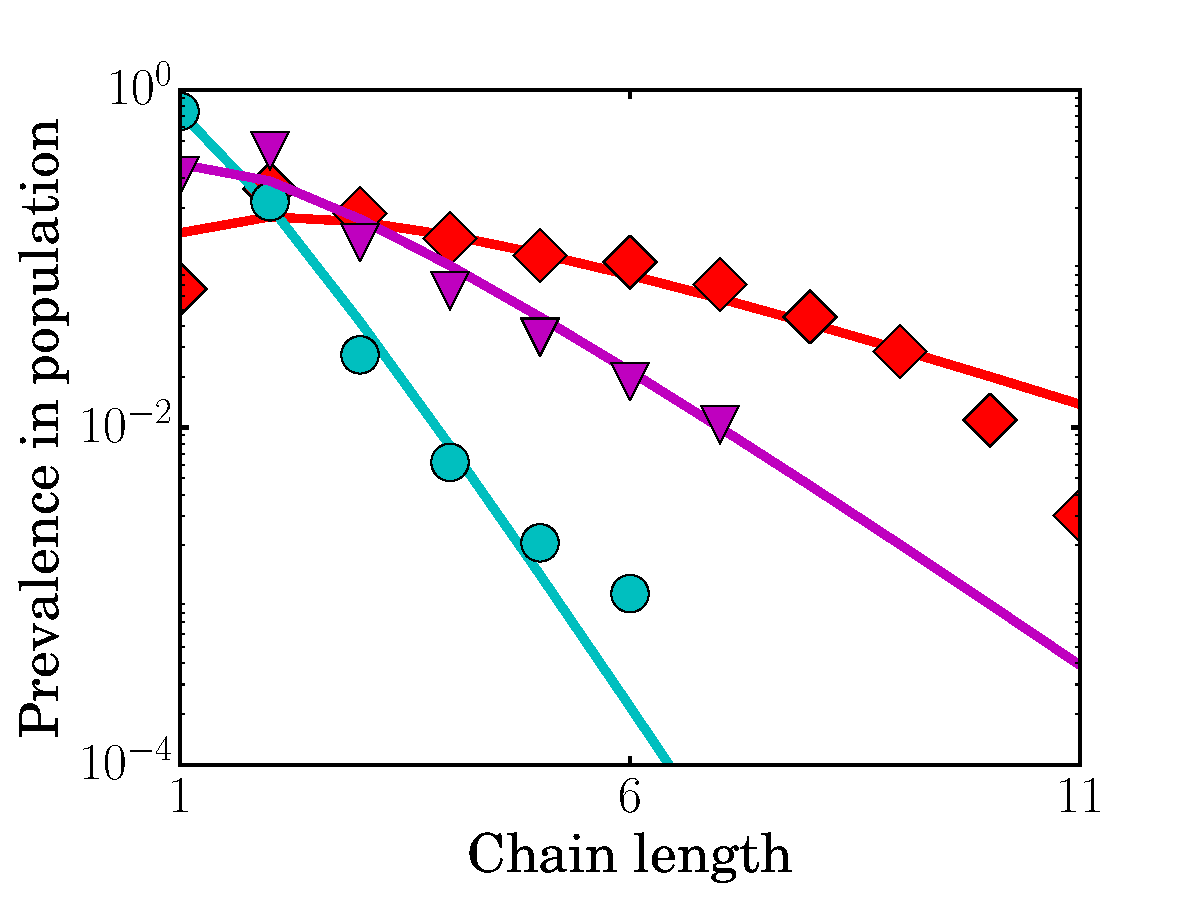
\includegraphics[width=0.9\columnwidth]{pictures/some_flory.pdf} 
%   \caption{\textbf{Prebiotic syntheses of peptides and nucleic acids lead approximately to the 
% Flory length distribution.}  }
%   \label{fig:some_flory}
% \end{figure}


\section{The foldamer-autocat mechanism: Short HP chains fold and catalyze the elongation of other 
HP chains}

 We propose that the key to the Chemistry-to-Biology transition may have been \emph{foldable 
polymers} (`foldamers').  Today's foldamers are predominantly proteins (Other foldamers include 
some RNA molecules and synthetic polymers\cite{Lee2005a}). Foldamers attain specific native 
conformations mainly through a binary solvation code of particular sequence patternings of the $H$ 
(hydrophobic) and $P$ (polar) monomers~\cite{Chan1991}.  We call these $HP$ copolymers.  It does not 
require a stretch of imagination to suppose that proteins, which are today's biological catalysts, 
could also have been primitive catalysts at the earliest stages.  Precision and complexity are not 
required for peptides to perform biological functions.  For example, proteins generated from random 
libraries can sustain the growth of living cells~\cite{Fisher2011}.  And, specific binding actions 
between random peptides and small molecules are not rare~\cite{Cherny2012}.  Below, we describe 
results of computer simulations that lead to the conclusion that short random HP chains carry within 
them the capacity to autocatalytically become longer and more protein-like.  Here are the premises 
of the model:
 
 \begin{itemize}
 \item [a.] A substantial number of random HP sequences, even of fairly short chains, will fold 
into compact structures resembling native or molten-globule proteins.
 \item [b.] Some HP foldamers will have exposed hydrophobic `landing pad' surfaces.
 \item [c.] Foldamer-autocats are HP sequences having landing pads. They can catalyze the 
elongation of other HP chains.
\end{itemize}

There are a few evidences that supports these premises.
\begin{itemize}
\item [a.] Non-designed random $HP$ sequences 
are known to fold.  $HP$ polymers have been studied extensively as a model for the folding and 
evolution of proteins~\cite{lau1989lattice,Chan1991,Miller1995,Yue1995,agarwala1997local}.  They 
show that stably folded structures of proteins can be explained predominantly by binary patterning 
of polar and hydrophobic residues, with finer tuning by specific interresidue 
contacts~\cite{Yue1992,Xiong1995}.  This view is supported by extensive experimental 
evidence~\cite{Lim1991,Kamtekar1993,Wei2003,Brisendine2015}. 

\item [b.]
We assume that HP foldamers have exposed hydrophobic surfaces and that they are sites of binding 
and catalysis. Such exposed hydrophobic clusters or patches are fairly common for 
real life proteins; their locations generally coincide with binding sites of ligands or other 
proteins~\cite{Lijnzaad1996}. These clusters are exploited in the recognition, binding of 
substrates and 
increasing rate of catalysis~\cite{MitchellGuss1983,Lijnzaad1996,VanEe1997,Witt1998}. For example 
hydrophobic clusters on the surface of lipases serve as initiation sites where the hydrophobic 
tail of a surfactant interacts with the patch first~\cite{VanEe1997}. A hydrophobic 
cluster on Cytochrome-c 
Oxidase is not a recognition element, but does increase $k_{cat}$\cite{Witt1998}. A survey of 
hydrophobic patches on the surface of 112 soluble, monomeric proteins~\cite{Lijnzaad1996} showed 
that the largest patches average around $400$\textit{\AA}$^2$ but can range from $200$ to 
$1,200$\textit{\AA}$^2$. A recent study~\cite{Tonddast-Navaei2015} showed that modern proteins have 
many sites of interaction with other proteins, typically nearly a dozen partners.  and nearly 3/4 
of 
its surface having geometrical properties that are amenable to interactions. These sites of 
interaction are enriched in hydrophobes.

\item [c.] Modern cells elongate protein chains using 
ribosomes.  Ribosomes catalyze protein elongation using an RNA core~\cite{Nissen2000}.  So, what is 
the evidence that protein elongation could be catalyzed by proteins?  First, the basic peptide 
chain elongation process is a condensation and removal of a water 
molecule~\cite[chapter 3, p.~82]{Nelson2008}.  Dehydration reactions can occur in water if carried 
in nonpolar environments, such as on hydrophobic surfaces or 
vesicles~\cite{Manabe2001,Manabe2002}, which serve as protection of hydrolysis and catalysts.  
Moreover, in bacteria and fungi, peptides are commonly synthesized by proteins (nonribosomal 
peptide synthetases) in the absence of mRNAs~\cite{Stachelhaus1998,marahiel2009working}.
\end{itemize}

\section{The computational HP lattice model of folding and catalysis}

 The method of choice for studying sequence-space properties of HP foldamers is the 2D lattice 
model~\cite{lau1989lattice,Chan1991}.  For example, that model led to the finding that a 
non-negligible fraction of the space of random sequences can collapse into compact structures 
resembling native proteins~\cite{lau1989lattice}; see fig.~\ref{fig:hydro-effect}.  While the 
2-dimensional HP lattice model entails obvious simplifications, it has the advantages that: (1) it 
is currently the only model that can explore full sequence and conformational spaces without 
parameters or bias, and (2) it is known to reproduce key observations on real proteins in 3D. The 
reason that the dimensionality is not problematic is because the determinative physics is in the 
surface-to-volume ratios of HP chains collapsing in water, and the 2D model for 12-25-mers in 2D is 
the same as that of 100-200-mer proteins in 3D~\cite{Giugliarelli2000}.
\begin{figure}[h!]
  \centering
  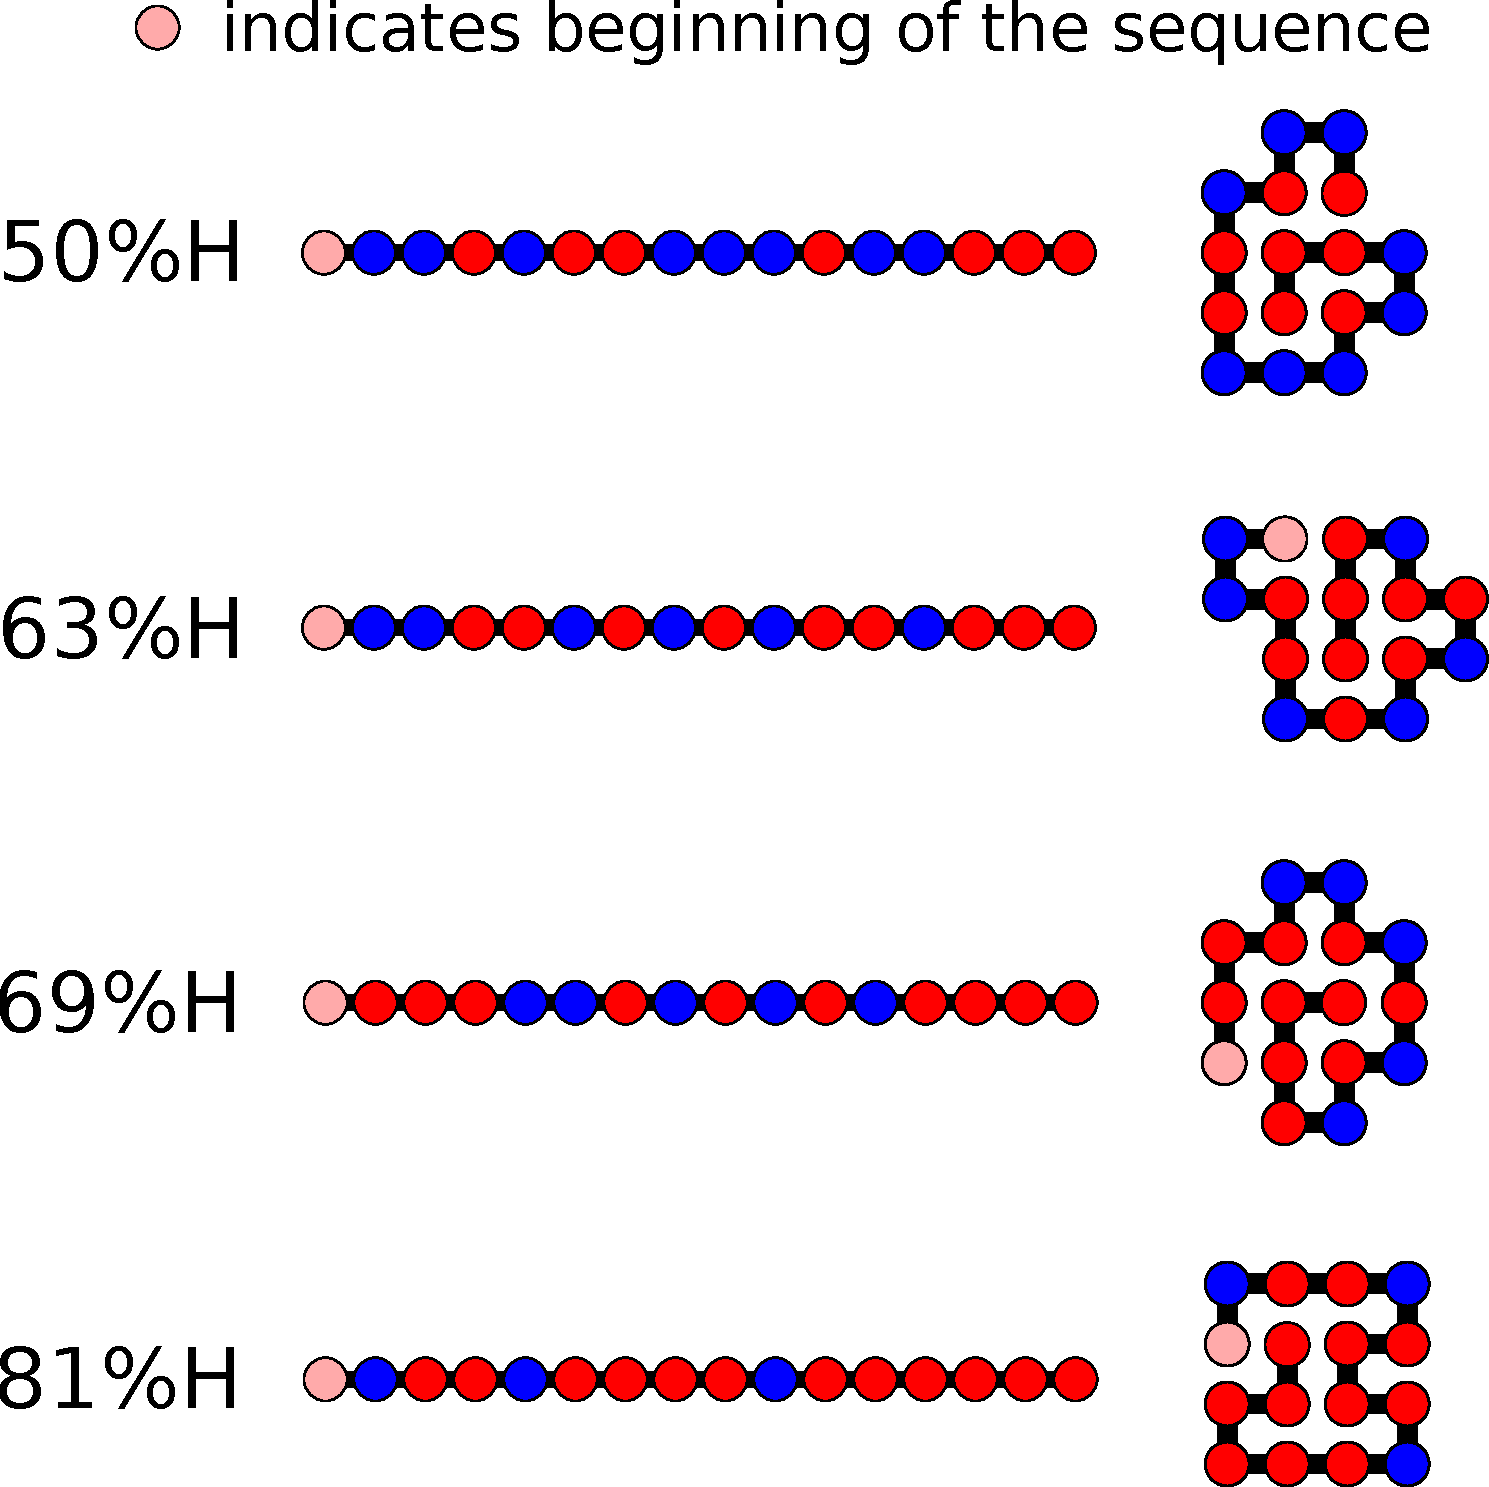
\includegraphics[width=0.8\columnwidth]{pictures/tst-seqs.pdf} 
  \caption{\footnotesize{HP sequences that fold to unique native structures in the HP 
lattice model.}}
  \label{fig:hydro-effect}
\end{figure}

 A central premise here is that some HP foldamers will have exposed hydrophobic surfaces that could 
act as primitive catalysts, as modern proteins do more optimally today.  Fig. \ref{fig:hp-catalysis} 
illustrates a commonly used mechanism of catalysts; namely translational localization.  A protein 
$A$ has a hydrophobic `landing pad' to which both a growing chain $B$ and a monomer $C$ will bind, 
localizing them long enough to form a bond that grows the chain.  How much rate acceleration could 
such a localization give?  Here's a crude estimate.  The free energy of a typical hydrophobic 
interaction is 1-2 kT.  If a folded polymer provides enough hydrophobic surface for a landing pad of 
3-4 hydrophobic interactions, this would reduce the kinetic barrier by 3-8 kT, will increase the 
polymerization rate by 10-fold - 3000-fold.  Of course, this rate enhancement is much smaller than 
the $10^7$-fold of modern ribosomes~\cite{Sievers2004a}, but it could have been relevant to 
prebiotic processes.
   \begin{figure}[h!]
  \centering
  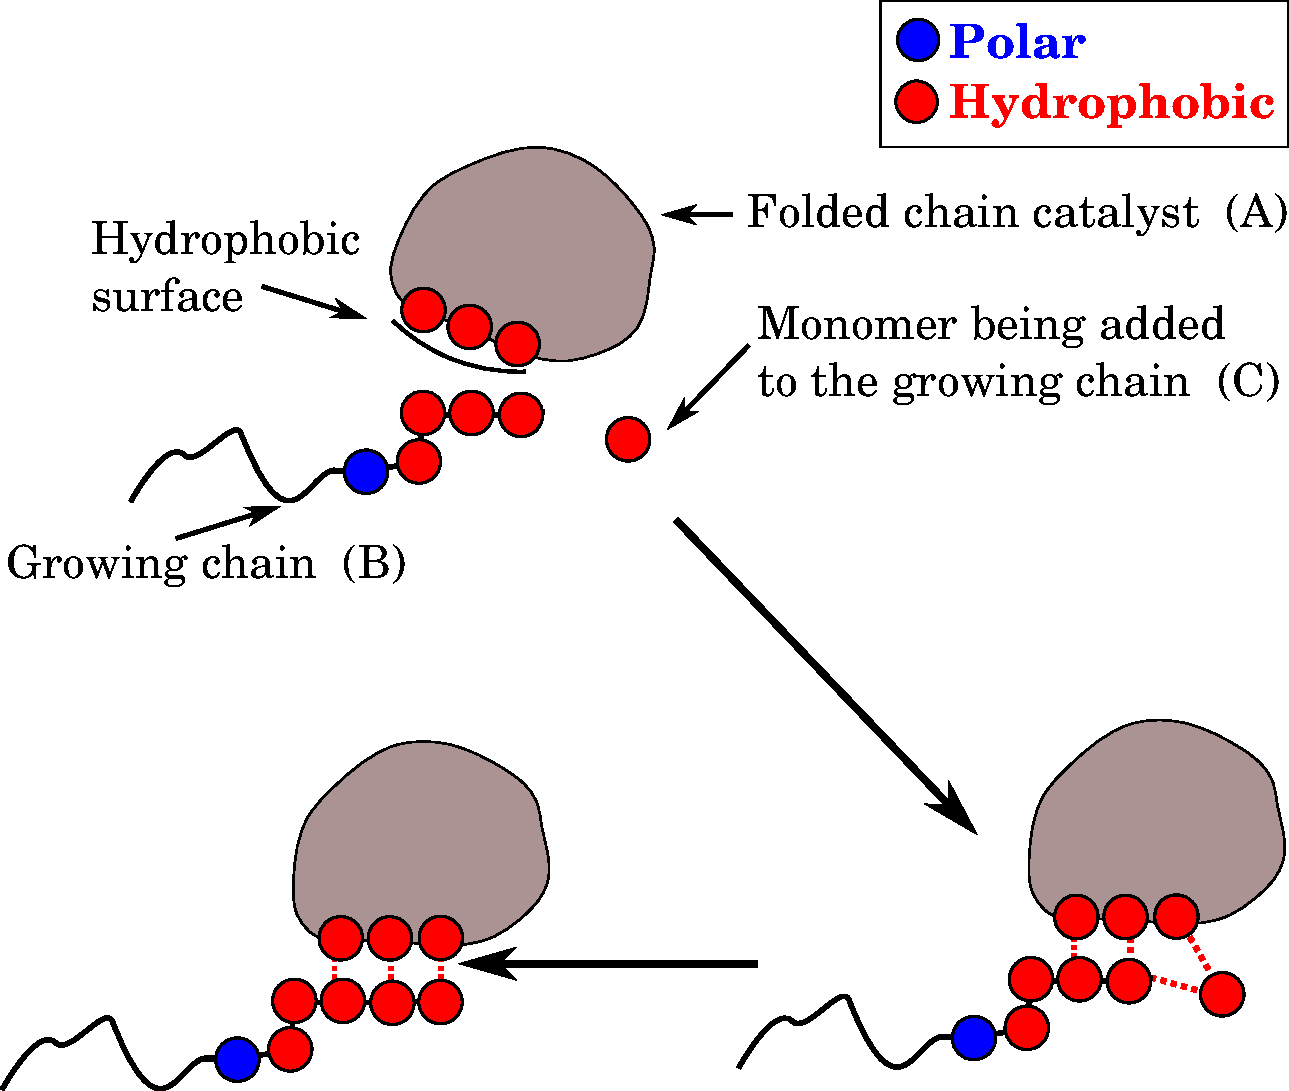
\includegraphics[width=0.8\columnwidth]{pictures/hp-catalysis.pdf} 
  \caption{\footnotesize{\textbf{Some HP foldamers have hydrophobic patches, which serve as 
landing pads that can catalyze the elongation of other HP chains.}  Chain $A$ folds and exposes 
hydrophobic monomers on its surface.   It serves as a sticky spot, or landing pad, for another $HP$ 
molecule $B$, in addition to an $H$ monomer $C$.  This localization action reduces the barrier to 
the polymerization of chain $B$ to monomer $C$.}}
  \label{fig:hp-catalysis}
\end{figure} 

 Here is the computational model we use.  We first describe the polymerization dynamics.  We 
consider a soup containing a sufficient supply of activated $H$ and $P$ monomers in solution.  Both 
current life and early life must be out-of-equilibrium.  In our modeling, that means that activated 
$H$ and $P$ monomers are supplied by an external source with rate $a$. To 
maintain steady state we allow any molecule to be , modeling removal of molecules from the 
system, 
say due to cell division or dilution.  A given chain elongates 
through an addition of a monomer, at rate $\ga$. Chains 
as well can undergo spontaneous hydrolysis due to interaction with watre; any bond can be 
broken with rate constant $h$. Without loss of generality we define the unit 
rate by setting $\ga = 1$.  All other rates are taken relative to this chain growth rate.   


 In addition, we include folding within the dynamical model.  We regard an HP sequence as folded if 
it has a unique lowest-energy `native' structure (a single conformation having the maximum possible 
number of HH non-covalent contacts).  Relatively few random sequences fold uniquely.  Most HP 
sequences either don't fold at all (i.e. $PPP \ldots P$), or collapse only into multiple 
molten-globule-like states; we don't consider these to be foldamers.   
The conformational free energy of the native fold ($E_{nat}$) of any particular folded sequence 
equals 
the number of hydrophobic interactions ($n_{h\phi}$) $\times$ (the energy $E_H$ of one hydrophobic 
interaction), which is $\approx 1-2kT$~\cite{Ghosh2009}:
\begin{equation}
 E_{nat}=n_{h\phi}E_H.
\end{equation} 
This energy differs for different sequences.  Now, given knowledge of $E_{nat}$ for any particular 
sequence, we can readily estimate the folding and unfolding rate coefficients from~\cite{Ghosh2009}:
\begin{equation}
 \ln\pt{\frac{k_f}{k_u}}=-\gD G/kT = E_{nat}/kT-N\ln z,
\end{equation} 
for reversible folding, where $z$ is the number of rotational degrees of freedom per peptide bond. 
 
 As with modern proteins, folded and unfolded states are assumed to behave differently.  We suppose 
that a folded chain is prevented from further growth, and also are protected from hydrolysis.  This 
simply reflects that open chains are much more accessible to degradation from the solvent or 
adsorption onto surfaces than are folded chains.  Even so, folding in our model is a reversible, as 
it is for natural proteins, so some small fraction of the time even folded chains are unfolded, and 
in that proportion, our model allows further growth or degradation.   In the section Simulations, 
we describe the details of model of the dynamics of adding 
monomers to growing chains, across HP sequence space, their folding (or not), and their adsorption 
and elongation on folded HP chains.  The results of the simulations are given below.
 
 Finally, we also allow for the possibility of catalysis upon foldamer surfaces.  The catalytic 
enhancement of chain elongation depends on the barrier reduction by hydrophobic localization, 
according to $\ga\cdot\exp(E_{H}\cdot n_{c}/kT)$, where $n_c$ is the number of hydrophobes in the 
landing pad (see figure \ref{fig:fold-cat}).  We take the minimum size of a landing pad to be 3.  
So, wherever three contiguous $H$ monomers are displayed on the surface of a stable foldamer, that 
molecule is a catalyst for elongation of other chains.
 
\section{Results}
\begin{figure*}[h!]
  \centering
  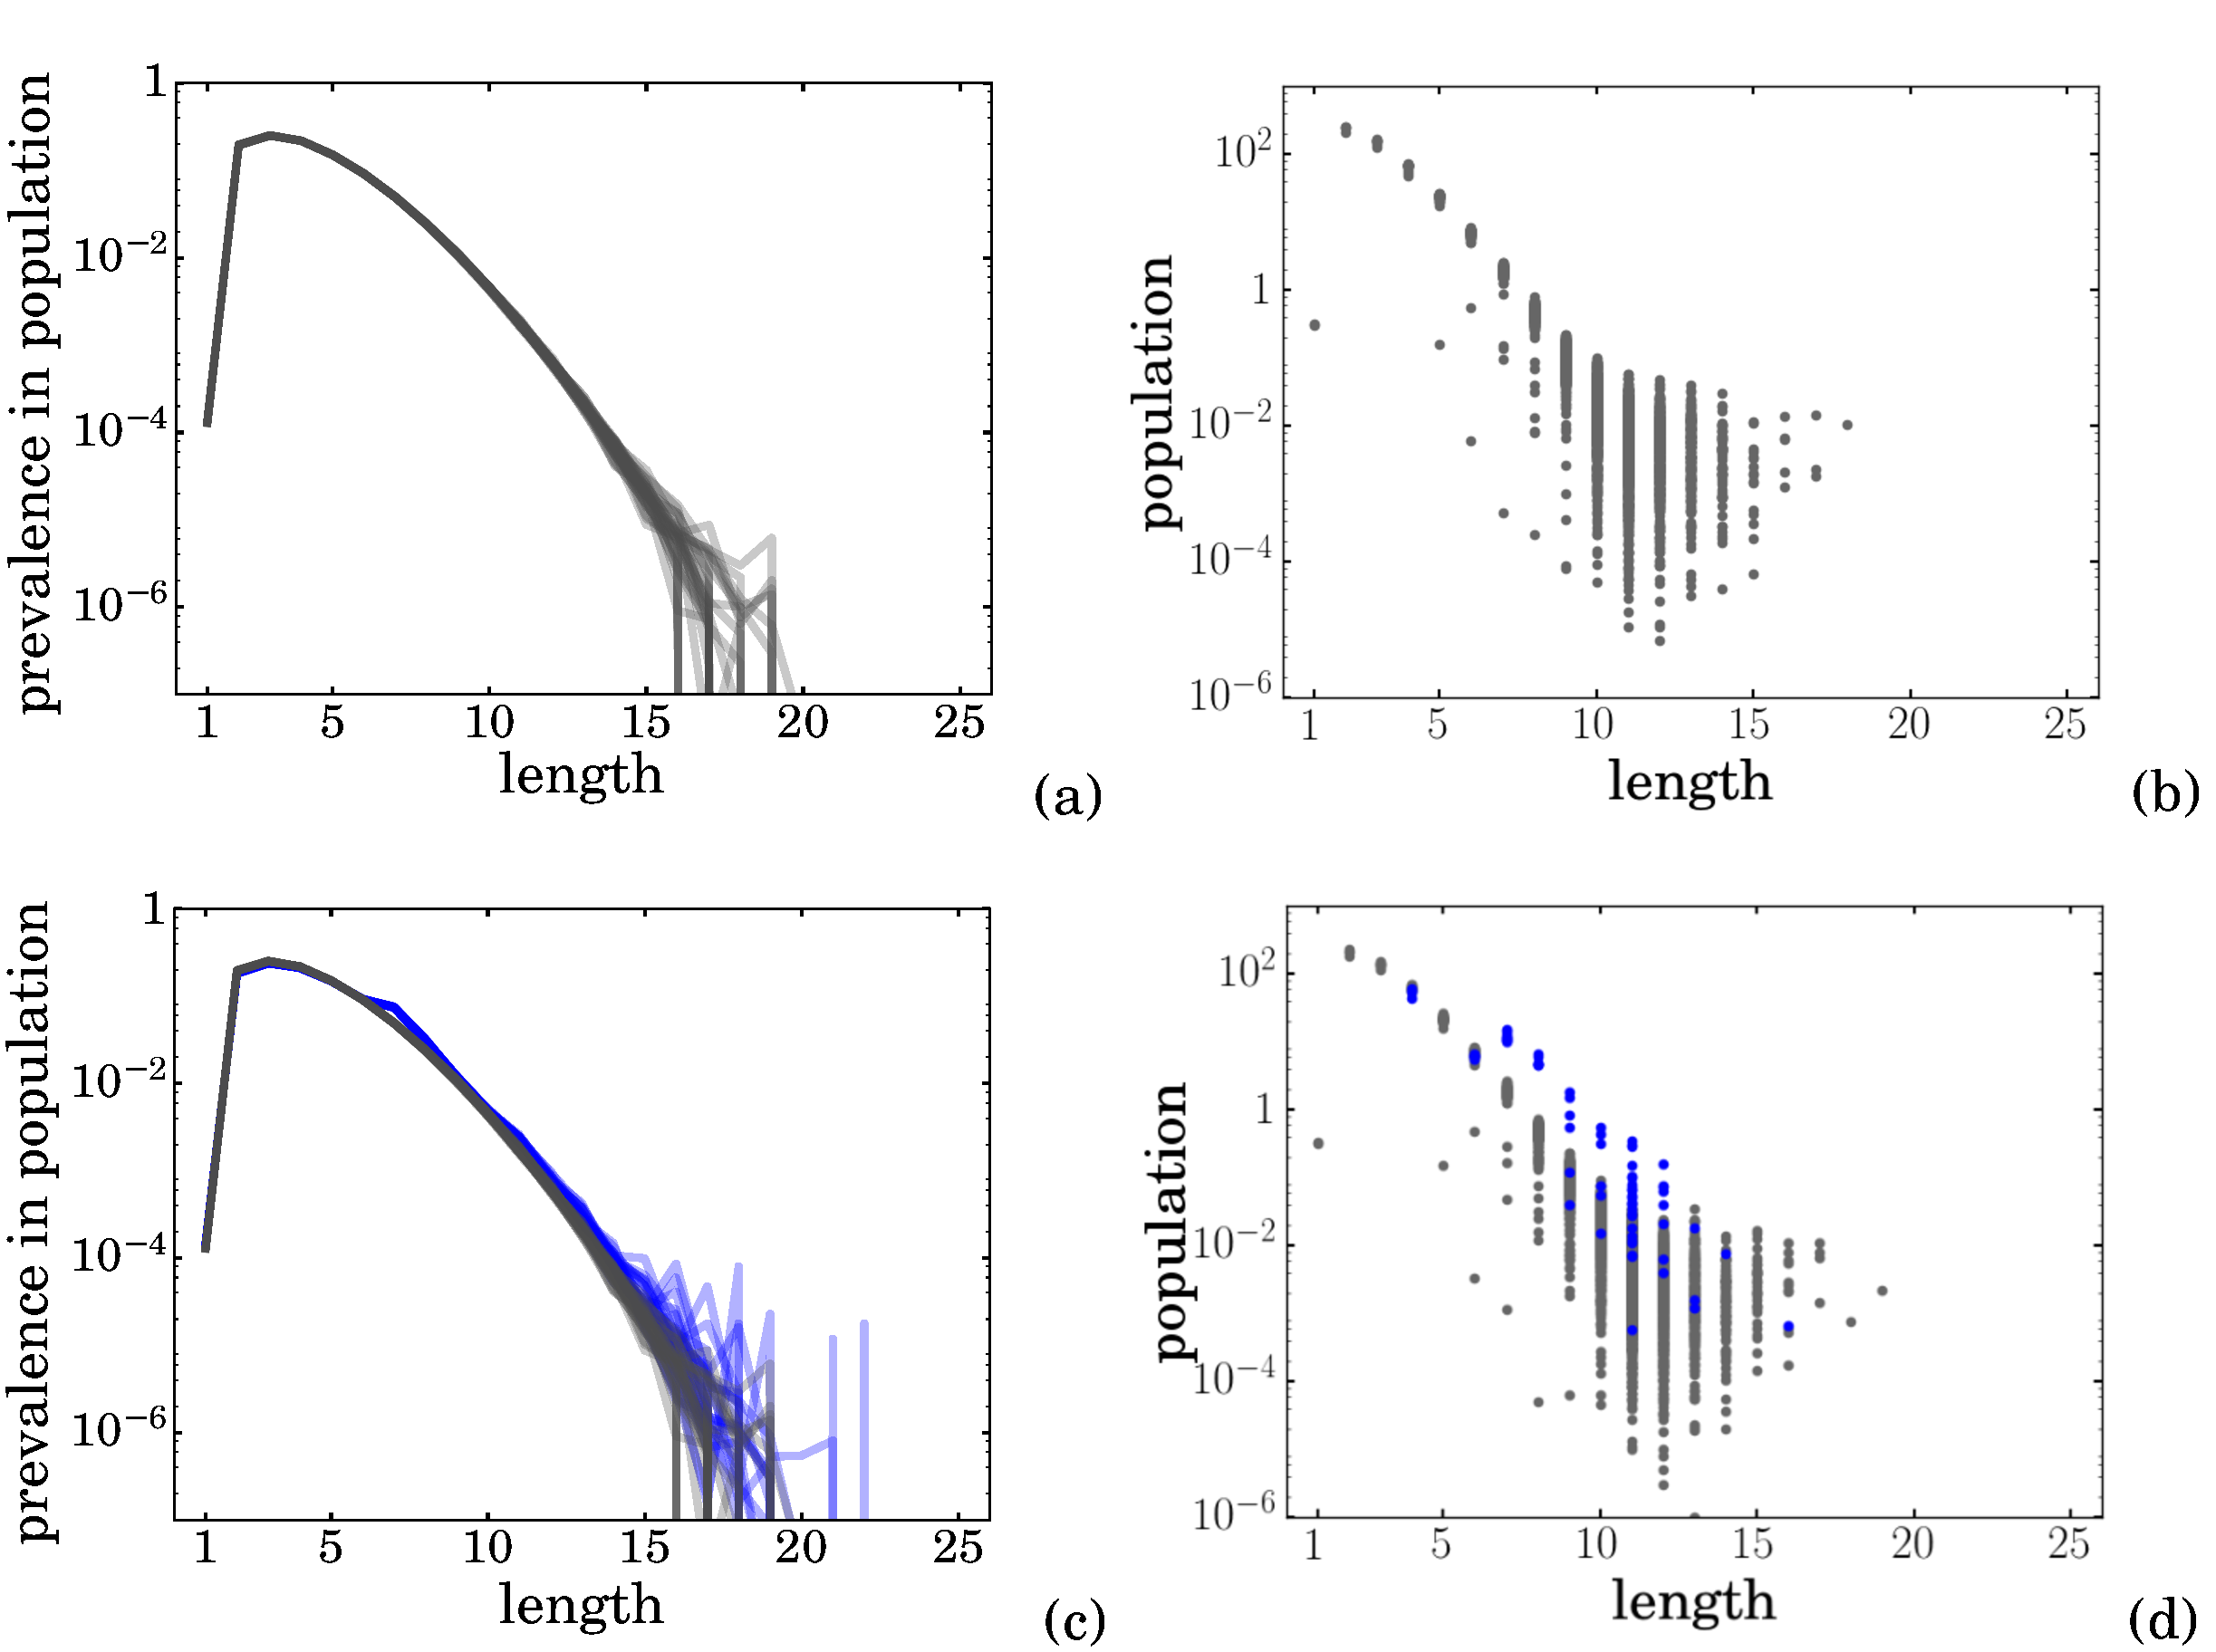
\includegraphics[width=0.9\textwidth]{pictures/distr-many-not-good.pdf}
%     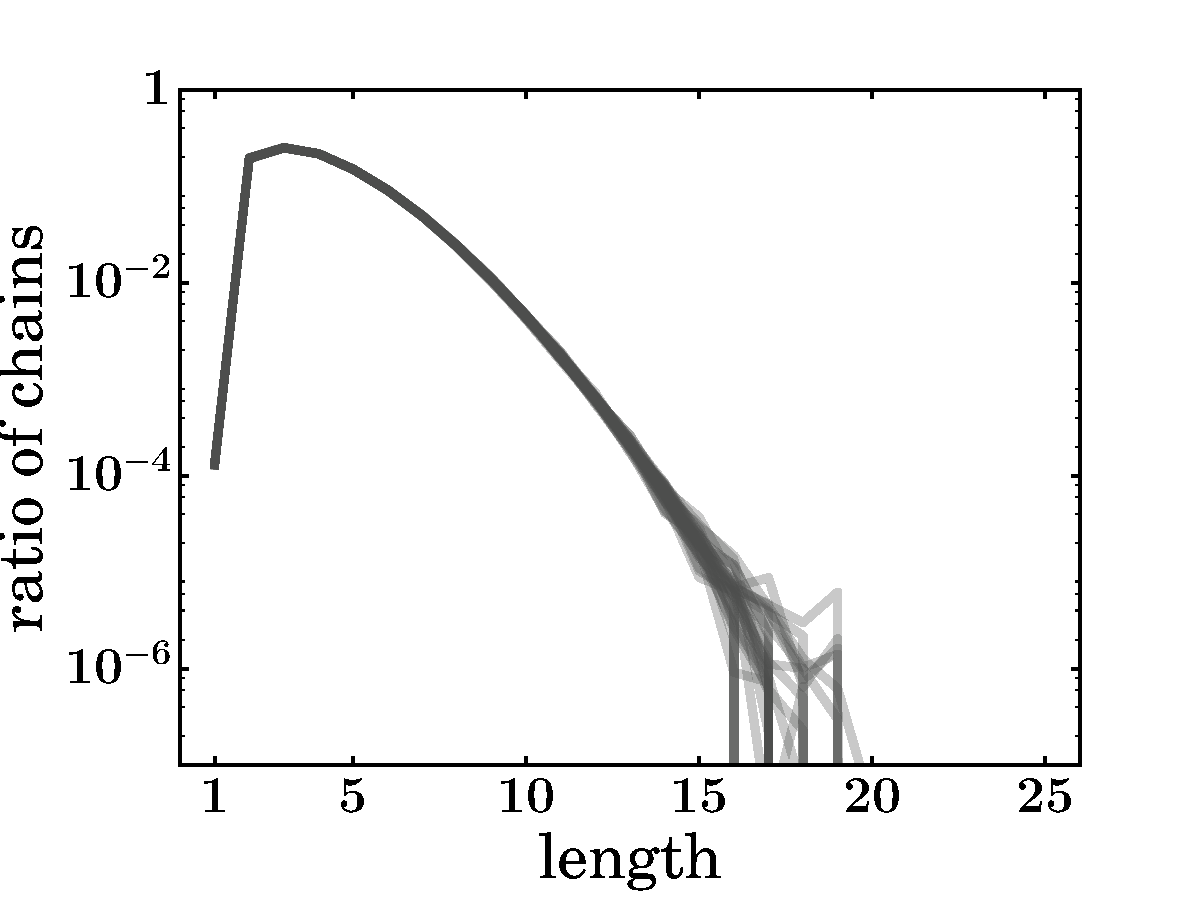
\includegraphics[width=0.45\textwidth]{pictures/distrPlain-many.pdf} (a)
%   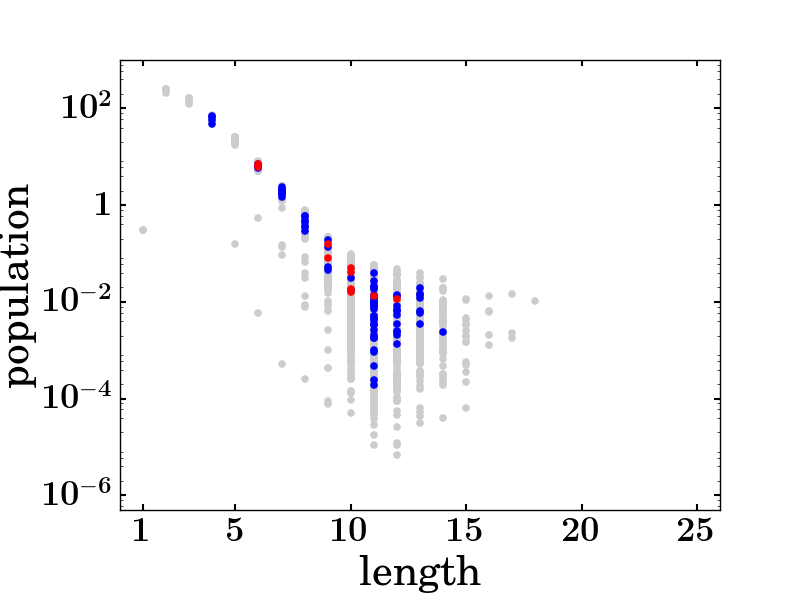
\includegraphics[width=0.45\textwidth]{pictures/scatter01918.png} (b)\\
%   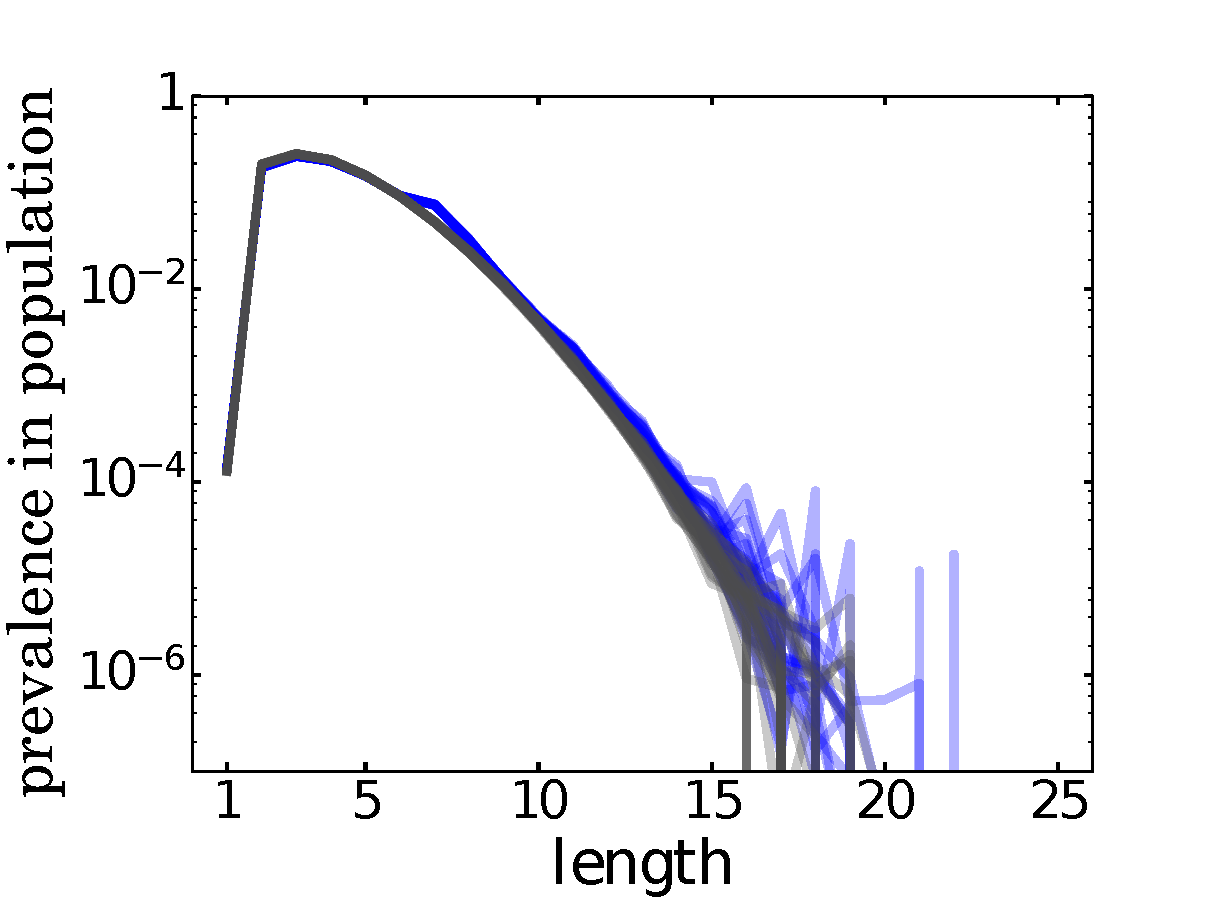
\includegraphics[width=0.9\columnwidth]{pictures/distr-folded-many.pdf} (c)
%    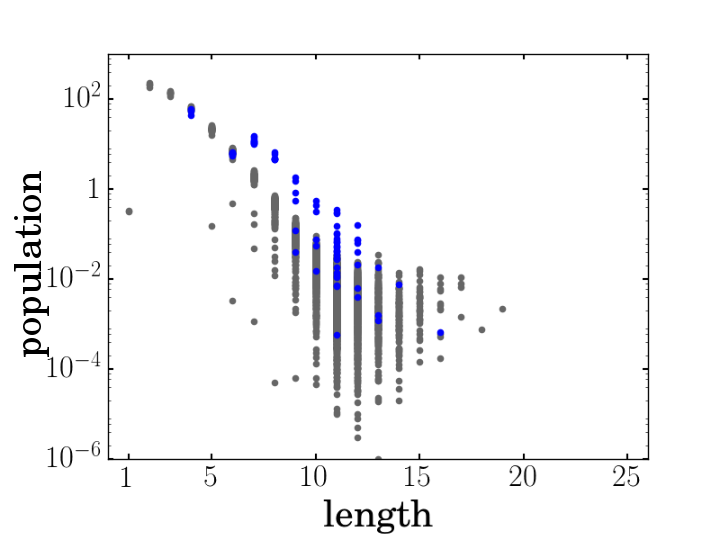
\includegraphics[width=0.9\columnwidth]{pictures/scatter2009.png}(d)
  \caption{\footnotesize{
\textbf{Experiment 1.  Reference test without folding or catalysis, the model gives 
the Flory distribution.  Average over sequence space (a,b).}  (a) A single line shows the length 
distribution for one simulation run with total of 30 lines corresponding to 30 simulations. 
 (b) Some particular sequences. Each point on the graph represents a population of an
individual sequence, based on the results of a single simulation run. Each data point on both 
panels is a result of averaging across $10^6$ time points in the steady state interval.   
    \textbf{Experiment 2: HP polymerization and folding, but not 
including catalysis.  This, too, only gives the Flory distribution (c,d).}  Each data point is an 
average of $10^6$ time points in the steady state interval. (c) 
A single line shows length distribution for one simulation run (we run total of 30 simulations). 
Blue lines are result of the Experiment 2, gray ones -- Experiment 1. Addition of folding to the 
basic model doesn't change the nature of distribution. (d) Populations of the individual 
sequences, 
based on the results of a single simulation run. Here we have two types of sequences: the ones 
which can fold are depicted as blue, and the ones which can't as gray. Foldable sequence have 
advantage compared 
to unfoldable ones.}}
  \label{fig:sim.flory-fold}
\end{figure*}
 First, we performed some reference-state tests.  We first `turned off' folding and catalysis by 
setting the hydrophobic energy to $0$ (see Experment 1, Section \ref{sec:experiments}).  Figure 
\ref{fig:sim.flory-fold}(a) 
shows that, as expected, this model captures the Flory model length distribution, having an 
exponential tail.  Figure \ref{fig:sim.flory-fold}(b) illustrates distribution within each length: 
gray dots represent individual sequences in a randomly chosen realization of the experiment. 


\subsection{Folding alone does not solve the Flory Problem}
 Second, we tested whether HP chain folding alone would be sufficient to bend the Flory length 
distribution curve (see Experiment 2, Section \ref{sec:experiments}).  If a chain folds, it 
protects its interior 
residues from 
hydrolysis.  Is this protection from folding sufficient to lead to longer chains?  
Figure~\ref{fig:sim.flory-fold}(c,d) shows that the answer is no.  In our model, chain folding 
alone is 
not sufficient to escape the Flory problem of the exponentially diminishing concentrations of longer 
chains.  Folding does increase the abundances of some foldamers, but they are too rare to affect the 
whole distribution.



\subsection{Modeling shows that HP foldamer-catalysts can solve the Flory Problem}
\begin{figure*}[htb!]
  \centering
  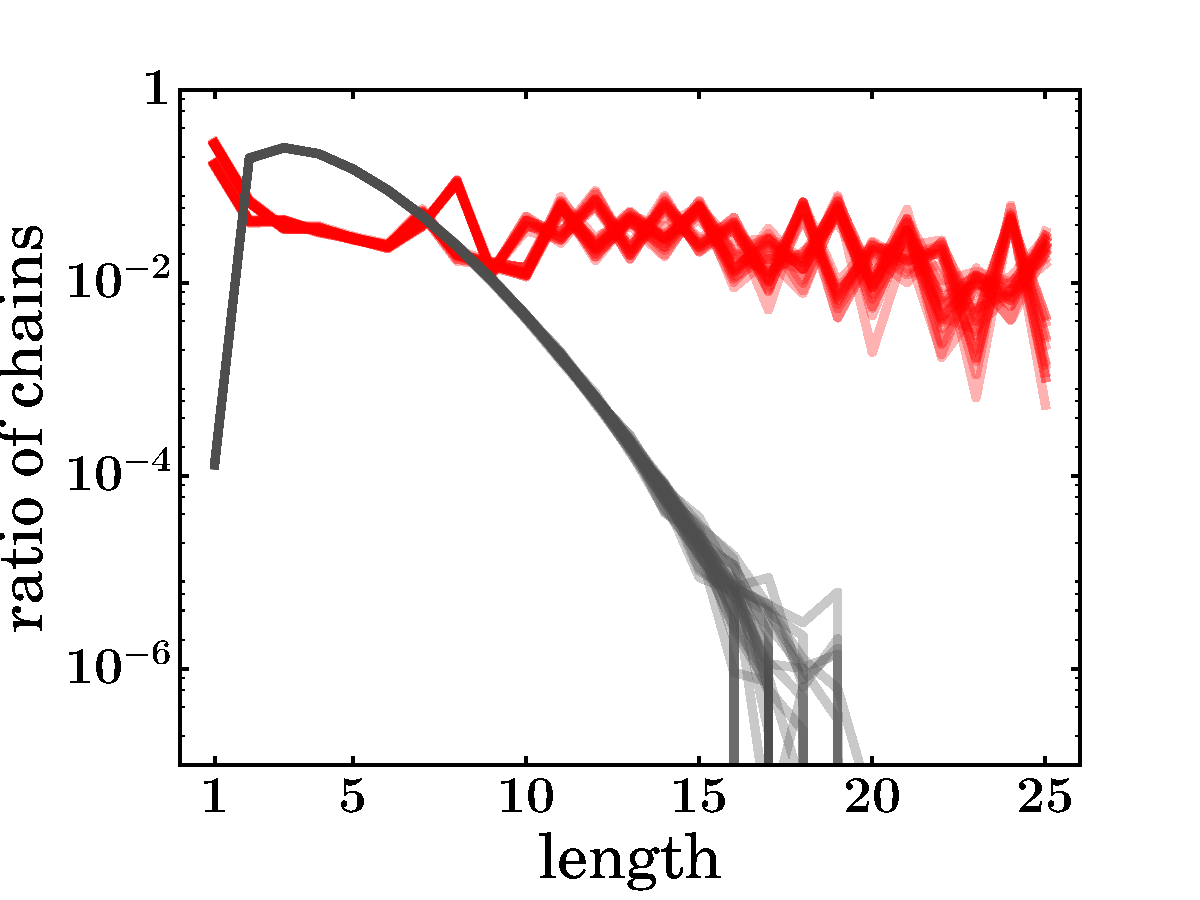
\includegraphics[width=0.9\columnwidth]{pictures/distrHP-plain-many.pdf}(a) 
  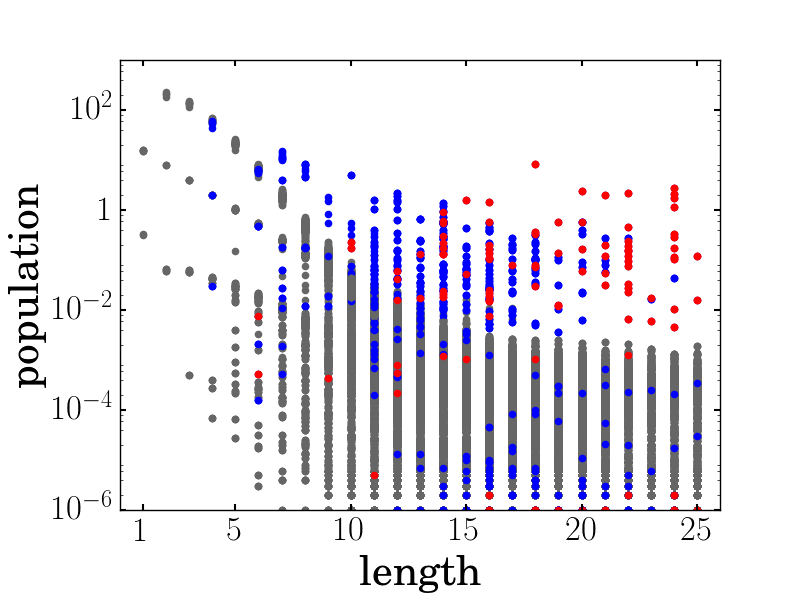
\includegraphics[width=0.9\columnwidth]{pictures/scatter1837.png}(b) 
  \caption{\footnotesize{\textbf{Experiment 3: Because some HP chains are foldamer-catalysts, it 
bends the Flory curve, giving an amplification of longer chains.}  Each data point is an average 
of 
$10^6$ time points in the steady state interval. (a) Gray lines represent polymerization without 
folding or catalysis. Red ones corresponds to a simulation run with folding and catalysis. A 
single 
line shows length distribution for one simulation run (we run total of 30 simulations). For 
details 
of simulations see section \ref{sec:experiments}, Experiment 3. (b) Populations of individual 
sequences are 
shown as 
functions of their length. Autocatalytic sequences are shown in red, sequences that can fold but 
cannot act as  catalysts -- in blue, and all the other sequences in gray. Lower limit of $10^{-6}$ 
is due to computational precision -- there are $10^6$ time steps over which we calculate average 
to 
get a point on the graph. Therefore the minimum possible population correspond to the case when 
sequence appeared only for one time instance. The data is an example based on one simulation}}
  \label{fig:stats-scatter-018}
\end{figure*}
Third, we tested whether accounting for both folding and catalysis could bend the Flory length 
distribution (see Experiment 3, Section \ref{sec:experiments}).  Figure~\ref{fig:sim.flory-fold} 
shows that it does. 
 The 
catalysis capability skews the length distribution significantly, independently of hydrolysis and 
dilution parameters, over about an order of magnitude in their range.  This is a main result of this 
paper:  Some HP chains fold, expose some hydrophobic surface, and therefore can reduce the barrier 
to elongation of other HP chains, leading to longer chains.  Figure \ref{fig:fold-cat} shows that 
this also results in an autocatalytic set: all foldamer-autocat HP sequences can catalyze the 
elongation of each other.
\begin{figure}[htb!]
  \centering
  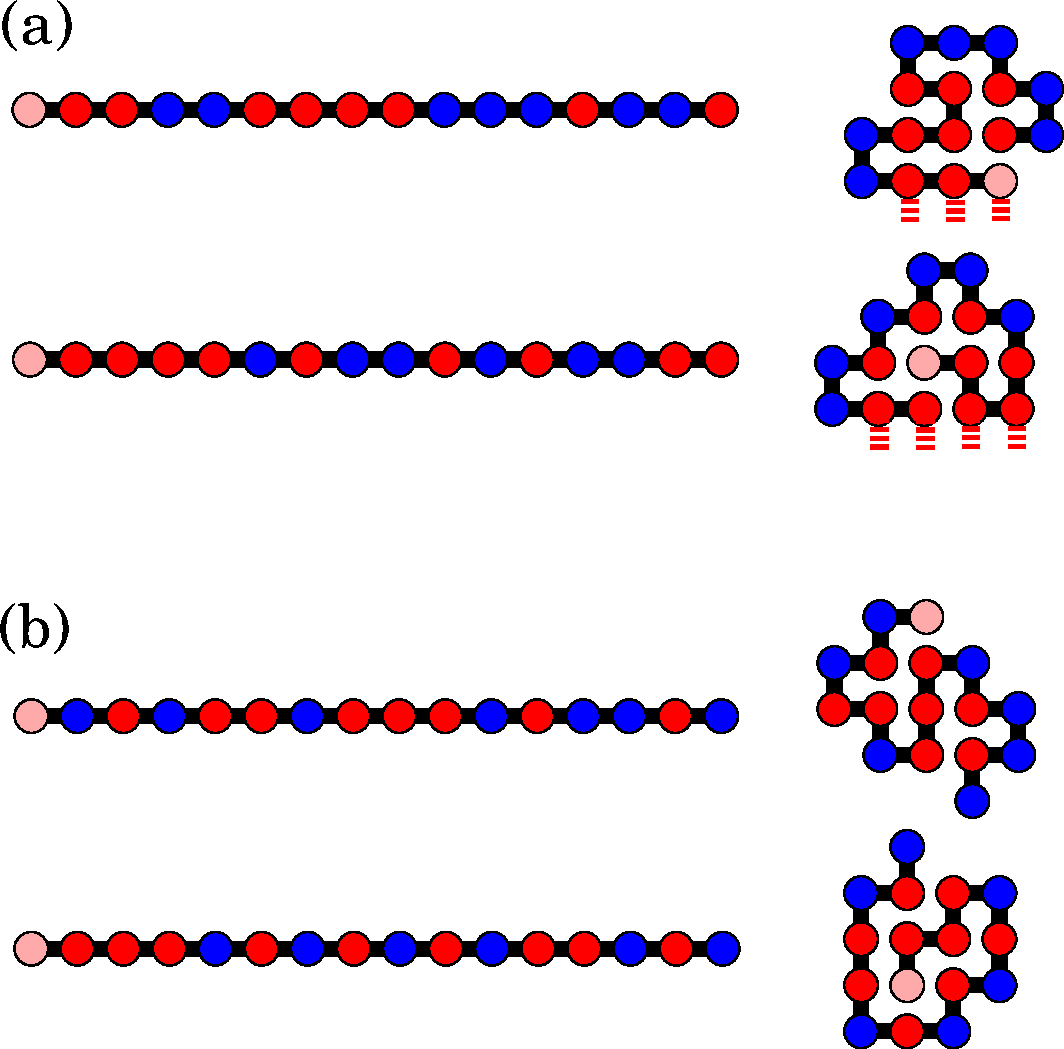
\includegraphics[width=\columnwidth]{pictures/fold-cat.pdf} 
  \caption{\footnotesize{\textbf{(a) HP lattice chains that fold and are autocatalytic.}  They fold 
into unique structures and have landing pads that can catalyze the elongation of each other.  
\textbf{(b) HP chains that fold, but are not catalytic.}  Most chains are not catalysts, but the 
size of 
the autocatalytic set is non-negligible; see Fig.~\ref{fig:hp-statistics}.}}
  \label{fig:fold-cat}
\end{figure}

Figure\,\ref{fig:stats-scatter-018}(b) show populations of individual sequence as function of 
their 
length. Colors represent type of the sequence: red -- for autocatalysts, blue -- for foldable, 
gray 
-- for the rest. The distribution inside the length, as one can see is drastically different 
compared to the case with folding only and without folding at all. For those cases, populations, 
while having large spread, 
are still clustered near average -- the typical $n$-mer is close to mean. When we introduce 
catalysis, 
there is no typical member anymore, there are many (often more than  50\% of all $n$-mers) 
sequences with very low populations and few with very high ones. In fact, the distribution within 
length is polynomial. Autocatalysts alone constitute a minority of the sequence space ( 
$\approx 
0.6\%$ 
of all the represented in the experiment sequences; foldable but inactive sequences occupy 
$\approx 
2.3\%$, regular sequences -- $\approx97.1\%$), however their contribution to the total mass is 
impressive: 
$\approx 15.7\%$; inactive folders -- $\approx 29.2\%;$ regular sequences $\approx 55.1\%$. 
Moreover, the longer the chain length, the higher the input of autocatalysts into total mass of 
that length (see figure \ref{fig:biomass}). This happens first of all due to increasing number of 
autocatalysts among longer sequences (see fig.\ref{fig:hp-statistics} and also due to the fact 
that 
folding along isn't capable of reaching longer chains. While at the shorter chains preservation 
from hydrolysis by means of folding is enough at longer chains active influence of catalysis is 
necessary. Average hydrophobicity of those sequences which dominate their length is $68\%$ (average 
is taken over 30 simulation runs in Experiment 3).
\begin{figure}[h!]
  \centering
  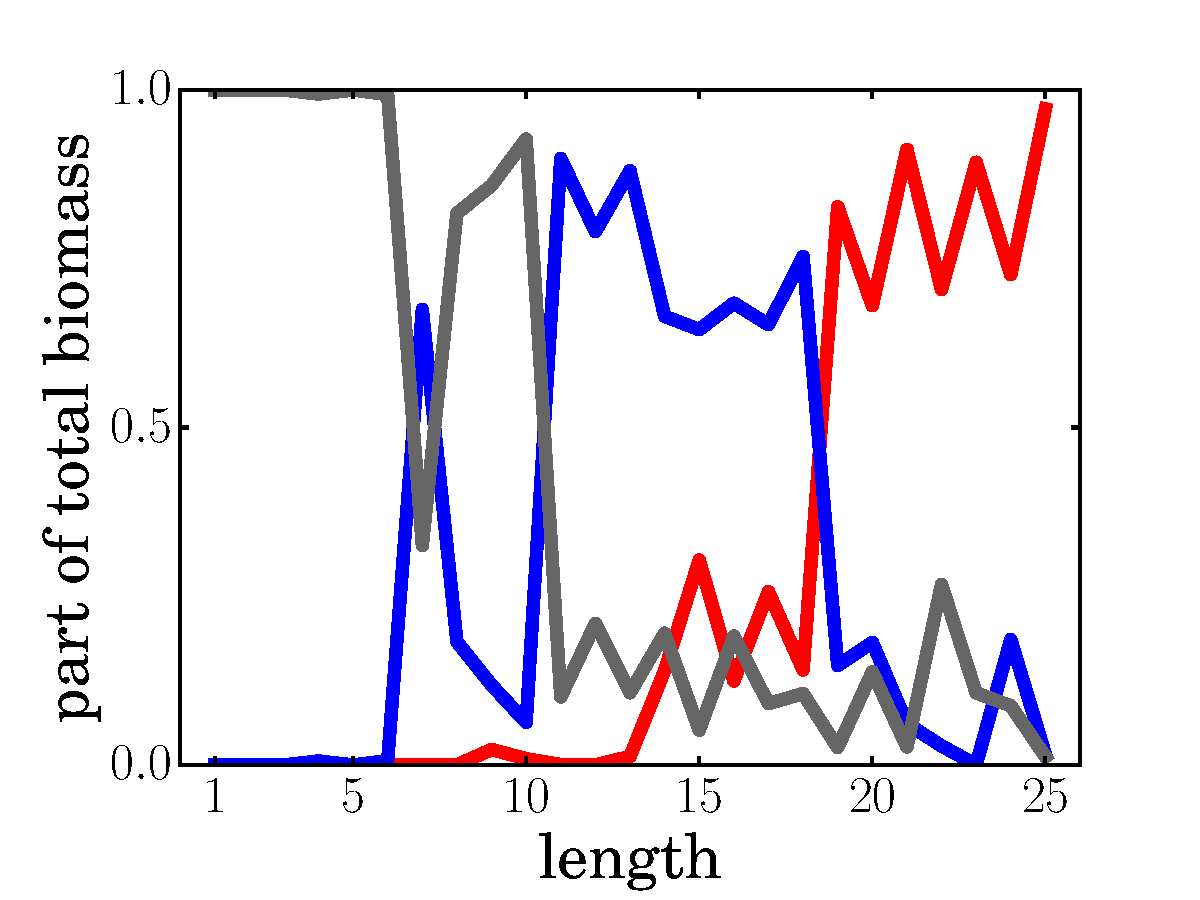
\includegraphics[width=0.9\columnwidth]{pictures/biomass.pdf} 
  \caption{\footnotesize{A single red line shows what ratio of the biomass of the 
given length is due to autocatalysts for a single simulation run. Each data point is an average of 
$10^6$ time points in the steady state interval. Black line is a median over 30 simulations }}
  \label{fig:biomass}
\end{figure}
\begin{figure}[hbt!]
  \centering
  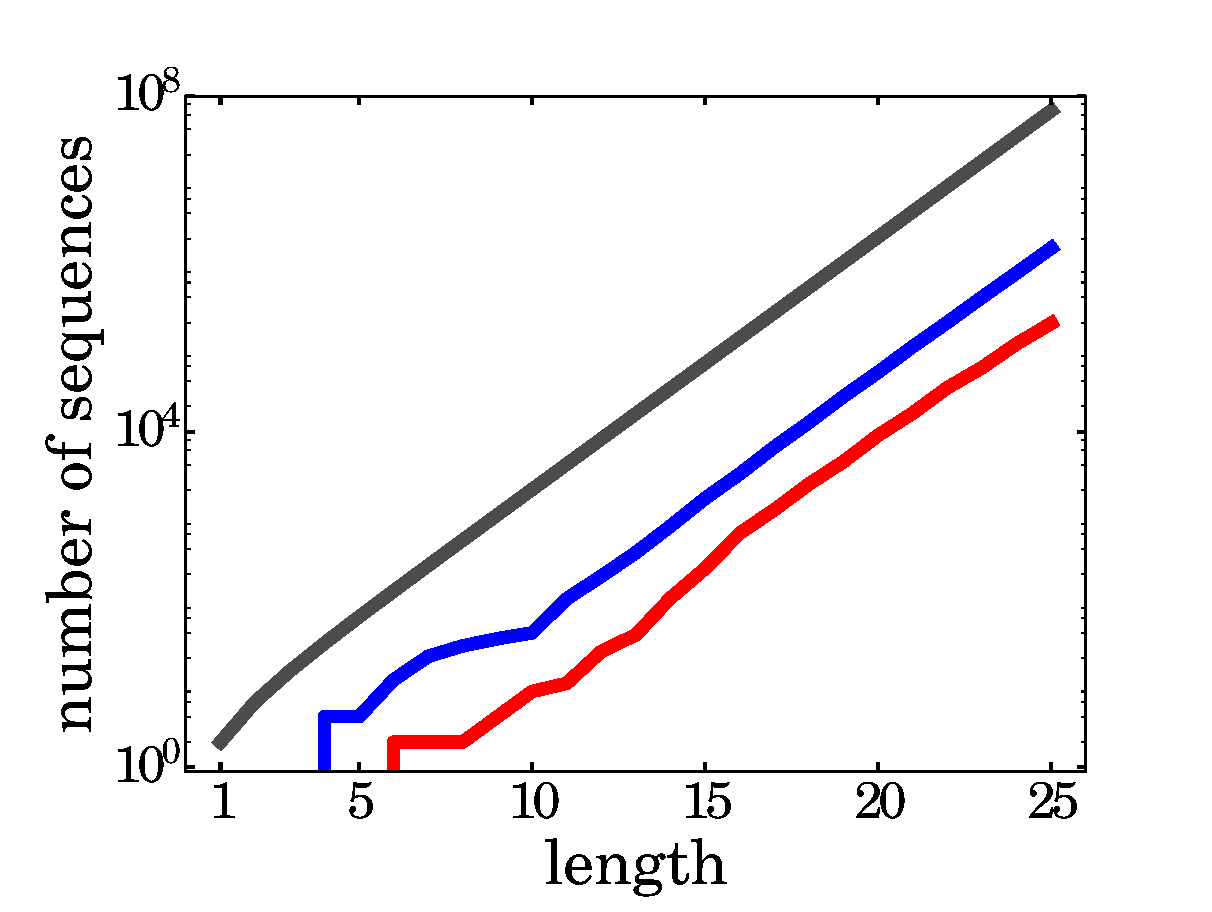
\includegraphics[width=0.9\columnwidth]{pictures/hp-statistics.pdf} 
  \caption{\footnotesize{The number of all HP sequences grows exponentially with chain 
length (gray).  The number of foldamers (blue) and foldamer catalysts (red) also grow 
exponentially.}}
  \label{fig:hp-statistics}
\end{figure}

At this point, we note what our model is, and what it is not.  Our model is not intended as an 
 accurate atomistic depiction of a real catalytic mechanism.  It is a coarse-grained toy model, of 
which there will be variants.  The mechanism we explore here is the translational localization of 
the two reactants, polymer $B$ and monomer $C$, in the chain extension reaction.  And, while this 
model is 2-dimensional, extensive previous studies have shown that it captures many important 
principles of folding and sequence-to-structure relationships.  At the present time, this type of 
model is the only unbiased, complete and practical way to explore plausibilities of physical 
hypotheses such as the present one.

We note that the present model is not necessarily exclusive to proteins.  NA molecules are also able 
to fold in water, indicating differential solvation.  While our present model focuses on hydrophobic 
interactions, it is simply intended as a concrete model of solvation, that could more broadly 
include hydrogen bonding or other interactions.  So, while our 
analysis below is only applicable to foldamers, it is not limited to proteins.  The unique power 
that foldable molecules have for catalyzing reactions -- in contrast to other nonfoldable polymeric 
structures -- is that foldamers lead to precisely fixing atomic interrelationships in relative 
stable ways over the folding time of the molecule.  It resembles a 
microscale solid, with the capability that substrates and transition states can recognize, bind, and 
react to those stable surfaces. For example, serine proteases utilize a catalytic triad of 3 amino 
acids.  So, foldability in some type of prebiotic polymer, could conceivably have had a special role 
in allowing for primitive catalysis.  Here, we use a toy model to capture that simple idea, namely 
that a folded polymer can position a small number of residues in a way that can catalyze a reaction.



\section{Discussion}
\label{sec:evolution}
 It has been recognized that life's origins require some form of 
autocatalysis~\cite{Kauffman1986,Dyson1985,Eigen1978}.  But, what molecular structural mechanism 
might explain it?  Here, we find that autocatalysis is inherent in the following process (see 
Figure \ref{fig:kinExamples}):  HP polymers 
are synthesized randomly; a small fraction of those HP polymers fold into relatively stable 
compact 
states; a fraction of those folded structures provide relatively stable `landing pad' hydrophobic 
surfaces; those surfaces can help to catalyze the elongation of other HP molecules having foldable 
sequences.
\begin{figure}[h!]
  \centering
  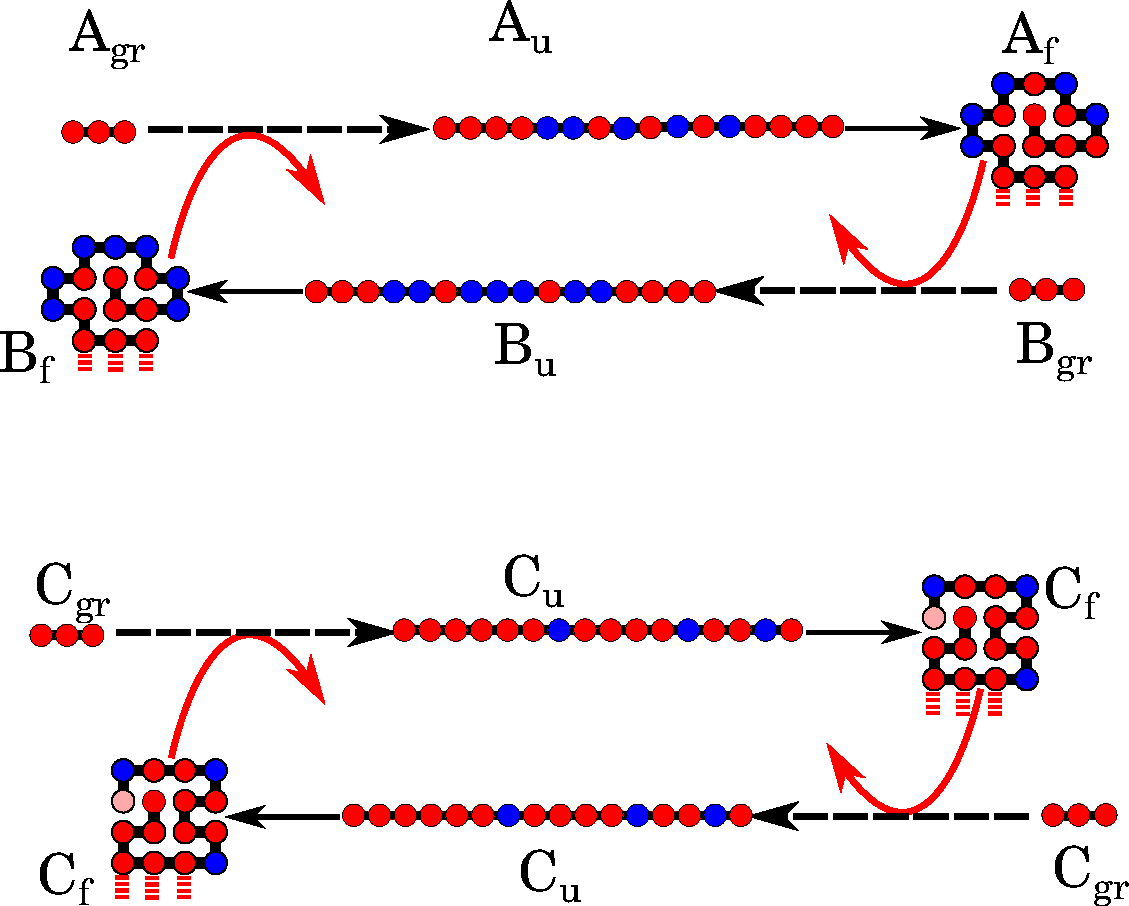
\includegraphics[width=0.9\columnwidth]{pictures/catalysis-kinEx-all.pdf}
  \caption{\footnotesize{Two examples of cross and autocatalytic interaction naturally embedded in 
HP-polymers dynamics. Dashed arrows (\textbf{-\,-\,-}) are shorten representation of multiple 
reactions of chain among which there are $\cdots HH - H$ catalyzed reactions. Catalysis is 
represented by red solid arrows (\red{\textbf{\textemdash}}). Solid black lines 
(\textbf{\textemdash}) are folding reactions. Chains, which we call ``autocatalytic'' experience 
catalysis during one (or more often several) of the steps of elongation. Then, when they reach the 
length at which they can fold ($A_u,\, B_u,\, C_u$), they fold and serve as catalysts them selves 
($A_f,\, B_f,\, C_f$). Mutual catalysis cat happen between different sequences (here A and B) and 
between different instances of the same sequence (here C).}}
  \label{fig:kinExamples}
\end{figure}

 The HP model allows for unbiased counting of sequences that do fold, don't fold, or fold and have 
a potentially catalytic hydrophobic landing pad.  A non-negligible fraction of all possible HP 
sequences fold to unique structures ($2.3\% $ for lengths up to 25-mers). The fraction of all 
possible HP sequences that have catalytic surfaces (as defined above) is $12.7\%$ of foldable 
sequences, or $0.3\%$ of the whole sequence space.  These ratios remain relatively constant with 
chain length, at least up to 25-mers; see figure \ref{fig:hp-statistics}.  This and successful 
designs of foldable, biologically active proteins based on the HP folding rule~\cite{Murphy2015} 
suggests that folding in HP polymers is not rare.  
   The present model provides an experimentally testable prediction for what early 
  polymer sequences could be autocatalytic, and provides a structural and kinetic mechanism for 
their action. 

Another interesting 
feature we observed in the $HP$ system is that in the presence of mutual catalytic activity it has 
a capacity for 
multiple quasistable states. Figure \ref{fig:distr1837-dyn}(a) shows two obvious ones.
Possible 
length distributions fall into two kinds, depending on random seed of the stochastic simulation. 
Both of these ``macrostates'' however correspond to a set of ``microstates'' characterized by a 
collection of several dominating autocatalytic chains. Thus presence of two stable distributions 
represents an emergent phenomenon in the system.
Whether particular sets of dominated sequences themselves constitute quasistable states is a matter 
of possible future investigation.

Nevertheless, one can notice a certain pattern in the ``microstates''.
Some of these dominating sequences are common to 
all microstates across both macrostates; they are likely to be important dynamical hubs of the 
system. Some sequences are common to the most of the microstates inside a certain macrostate; they 
appear to be a ``signature chains'' of this macrostate. Some sequences, on the other hand appear 
only once across all the realizations. 

It is possible that the system has not two but many quasistable states and thus it has a sequence 
variability and a potential for state switching.
Moreover, our system accounts for two 
types of monomers, yet in fact, in the case of proteins they correspond for 20 different amino 
acids, which of them have different hydrophobicities and can participate in slightly different 
reactions, thus, plausibly further increasing  number of stable states.
We believe that potential of the system for the multimodality worth further investigation to look 
for hints of possible adaptability.
Figure \ref{fig:distr1837-dyn}(b) shows the structure of the sequences, which \textit{most often} 
are main contributors into the total population of the polymers of their length. They are also 
notably far from the median population, with some exceptions: there are autocatalysts 
among 16mers (red) and 17mers (green), but none of them managed to emerge above median and aren't 
shown on the picture.
\begin{figure}[h!]
  \centering
  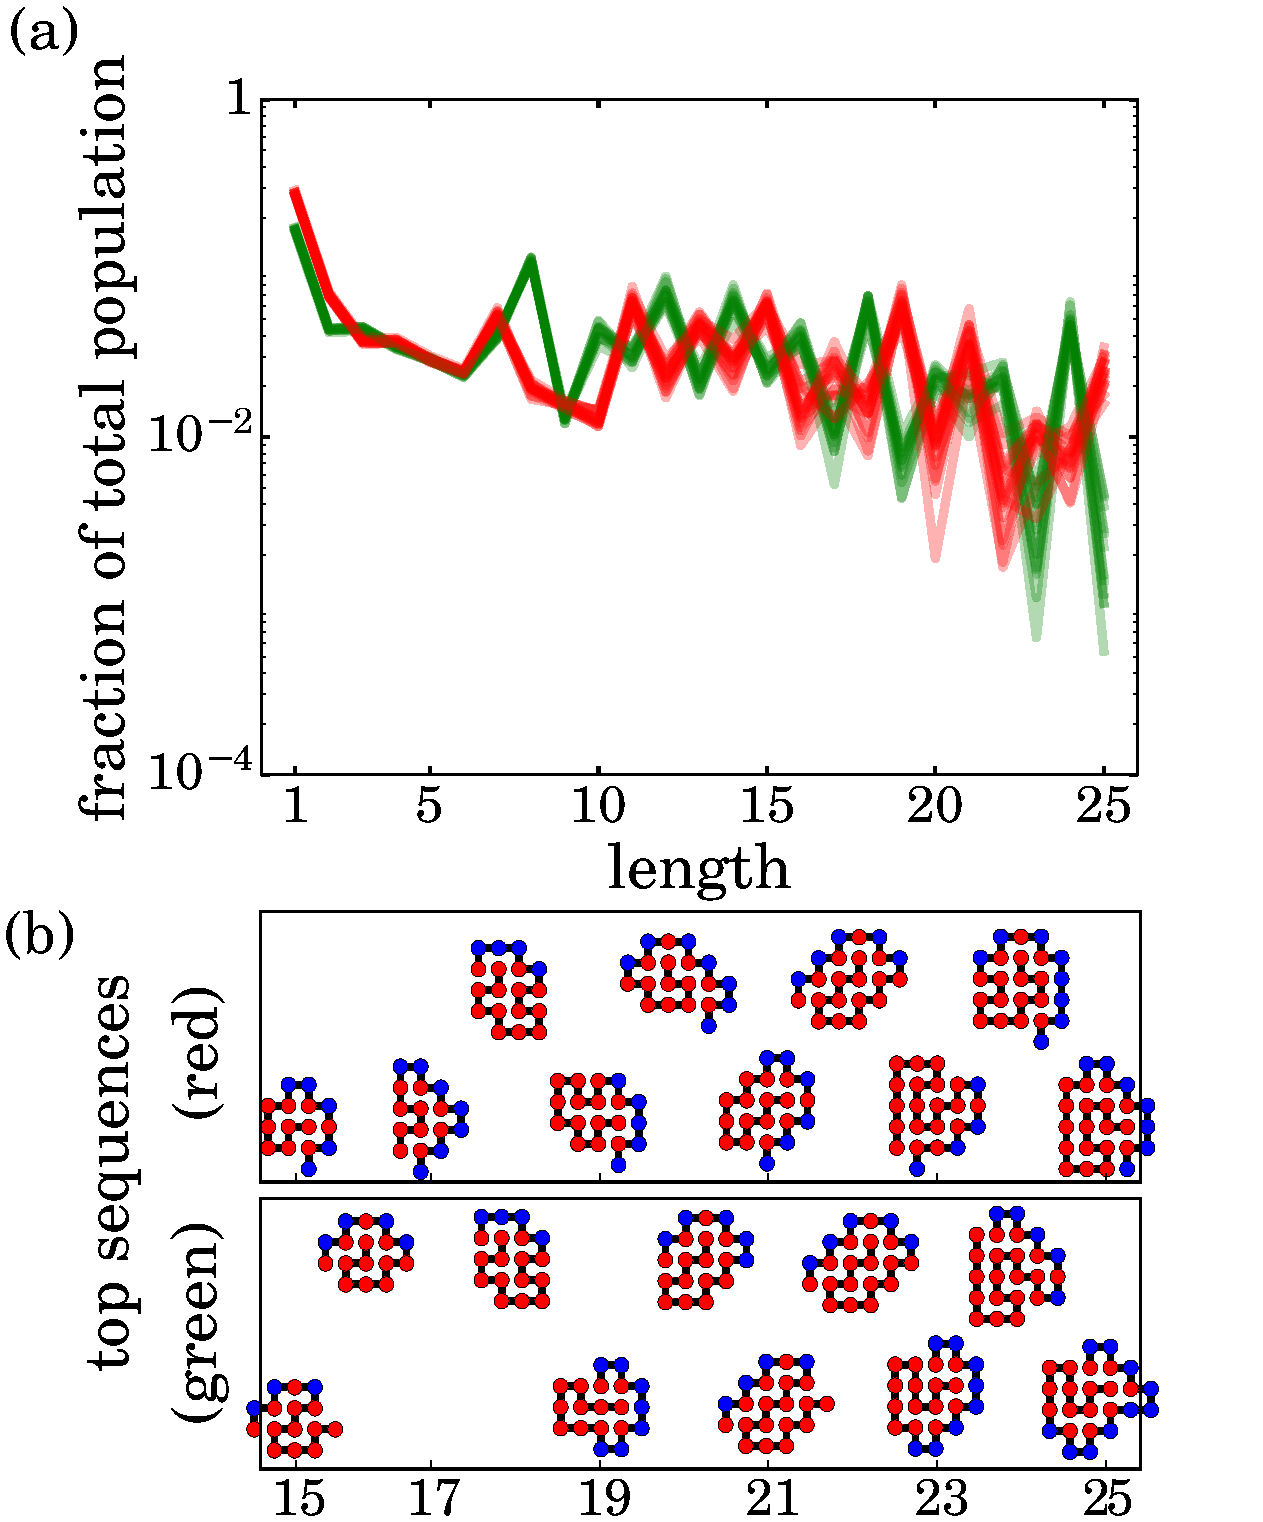
\includegraphics[width=0.9\columnwidth]{pictures/distr1837-dynamics.pdf}
  \caption{\footnotesize{\textbf{} (a) This figure shows that there the $HP$ catalytic system has 
at least two attractors. The lines are length distributions from Simulations, Experiment 3. Again, 
each line represents distribution of length in the steady state for one simulation run. It is 
clear, that there two kinds of distribution, which get realized during the simulations. System 
bifurcates either to a state represented by a green line or to one represented by red one. These 
are the same lines as on figure \ref{fig:stats-scatter-018}(a), but separated in two sets by a 
clustering algorithm K-means. (b) Structure of the sequences, which \textit{most often} 
are main contributors into the total population of the polymers of their length. Top panel 
corresponds to the macrostate shown in red on the panel (a), lower one, to the one shown in green. 
}}
  \label{fig:distr1837-dyn}
\end{figure}


 \section{Simulations}
We performed direct stochastic simulations.  This required development of appropriate simulation 
code because of the large numbers of different molecular species that we need to treat here.  We 
used Expandable Partial Propensity Method\footnote{The description and 
C++ library can be found at: https://github.com/abernatskiy/epdm.} (EPDM)~\cite{Guseva2016b}. The 
challenge for simulations is 
keeping track of all the molecular species and to search the full conformational spaces of each 
chain; this task is NP-hard.  We use the HP Sandbox 
algorithm\cite{lau1989lattice,Dill2008} \footnote{A Python implementation and description can be 
found at: http://hp-lattice.readthedocs.org/en/latest/}, which is 
limited to maximum chain lengths 
of 25.  To handle computational constraints, we 
limited the total number of species to the few 
thousands.  We impose this limit by introducing a dilution parameter $d$: molecules are randomly 
removed from the system with probability $\propto d$.  Physically, such This either can mimic a 
protocell splitting and loose of materials due to it or in the case when system isn't bounded by 
any 
borders the fact that some molecules will diffuse away. The total numbers of molecules vary within 
the range of $10^2-10^4$.

We start our simulations with a small pool of monomers, usually below 100 molecules. 

\begin{itemize}
 \item Monomers can be react with each other and with polymers to produce polymerization reaction 
with rate 
$\ga = 1$
\begin{equation}
 1\mbox{-mer}+n\mbox{-mer} \xrightarrow{\ga} (n+1)\mbox{mer}
\end{equation}
\item These monomers are being imported in the system. with rate $a\gg1$. It is safe to assume 
that 
we would have enough monomers in the system and import of monomers wouldn't be a bottleneck of 
reactions chain. Therefore we explore big values of $a\propto 10^3\ga$
\begin{equation}
 \emptyset \xrightarrow{a} H\,\,\mbox{or}\,\,P
\end{equation}
\item Hydrolysis has constant rate $h$ per bond. Half-life time of hydrolysis bonds in neutral 
conditions and temperatures around room temperature are on the order of hundreds of 
years\footnote{Hydrolysis rate constants of oligopeptides in 
neutral conditions are of the order of $10^{-11}-10^{-10}$: $1.3  10^{-10} M^{-1}s^{-1} $ 
for benzoylglycylphenylalanine ($t_{1/2} = 128 y$)\cite{Bryant1996}, $6.3  10^{-11} M^{-1} s^{-1}$
($t_{1/2}=350 y$) for glycylglycine and $9.3 10^{-11}M^{-1} s^{-1}$ for glycylvaline
\cite{Smith1998}.}. We test hydrolysis rate constants to be about $0.01-1$ of polymerization rate 
constants. This way we account for polymerization conditions, which happens on the order of days 
to years.
\begin{equation}
 n\mbox{-mer} \xrightarrow{h} l\mbox{-mer}+(n-l)\mbox{-mer}
\end{equation}
\item Dilution parameter $d$ mimics cell division and loss of the matter because of that. 
This parameter also serves utilitarian role of limiting total population of the cell. We explore 
valued of $d$ from $\propto 0.01\ga$ to $\propto 1\ga$. Given values of $a$ we'll explore various 
populations from $\propto 10^2$ to $\propto 10^4$ polymers per 
cell.
\begin{equation}
 \mbox{anything} \xrightarrow{d}\emptyset
\end{equation}
\item Folding and unfolding reactions happen very quickly with 
the unfolding rate constants of $k_f\gg k_{u}\gg\ga$. 
\begin{equation}
\begin{split}
 \mbox{folded chain}&\xrightarrow{k_u}\mbox{unfoled chain}  \\
 \mbox{unfoled chain}&\xrightarrow{k_f}\mbox{folded chain}
\end{split}
\end{equation}
The folding rate constant taken 
from~\cite{Ghosh2009}:
\begin{equation}
 \ln\pt{\frac{k_f}{k_u}}=-\gD G/kT = E_{nat}/kT-N\ln z,
\end{equation} 
 where $z$ is the number of rotational degrees of freedom per peptide bond.
 $HP$ model itself predicts only equilibrium constant, but not folding/unfolding rates.
 For those we had to rely on statistical models based on data on $k_f,\,k_u$ for 3D real life 
proteins~\cite{Ghosh2010,Dill2011}.
It helps that for our story actual precise numbers for these rates aren't necessary -- population 
of folded vs unfolded states is determined by equilibrium constant, so $k_f,\,k_u$ generally 
speaking can be any, as long as their ration is preserved. However it is important to keep proper 
time scales in the model. So we calibrated parameters taken from the literature so that yield 
unfolding/folding rates meaningful in the context of other rates in our model: folding is much 
faster than growth and for any of the sequence in our pool $k_f/k_u\in (10^2,10^4)$, which 
corresponds to empirical data~\cite{Ghosh2010,Dill2011} for 3D proteins.
However models mentioned are not sequence dependent and express only average rates. To keep our 
model sequence dependent, we set unfolding rate of all sequence to the average for their length 
and put all sequence dependence into $k_f$. Thus we used the following parameters. However it's 
worth noting that changing them in a rather wide range doesn't affect behavior of the system 
significantly.
\begin{equation}
\begin{split}
  k_u &= \exp[12-0.1 \sqrt{N} -E_H(0.5 N + 1.34)],\\
  k_f &= k_u\exp(\gD G)
\end{split}
\end{equation}

$E_h$ in our experiments is around $1-2$kT. $k_{unf}$ we keep $\propto 10^2$, which 
gives us range of unfolding rates from a reaction per hours and days and range of folding rates 
from a reaction per hours to fractions of a second.

\item Catalysis rate is proportional to the exponent of hydrophobic energy $E_h$ and number of 
contacting hydrophobes $n_c$: $\ga_{cat}=\ga\cdot\exp(E_{h}\cdot n_{c}/kT)$. Number of 
hydrophobic 
contacts 
for the short HP-sequences varies in the range $3-6$.Ther reaction is:
\begin{equation}
\mbox{Cat.}+H+ \underbrace{\cdots HH}_{l-1} 
\xrightarrow{\ga_{cat}}\mbox{Cat.}+\underbrace{\cdots HHH}
\end{equation}
 With the hydrophobic energies of $1-2$kT this gives us 
catalysis rates around hours and days for one reaction. Because the EPDM supports only binary 
reactions, we divided the reaction above into to steps: interaction of catalyst with a monomer 
with 
rate $\ga$ and reaction of this complex with a polymer with the rate $\ga_{cat}$. 
\end{itemize}

We investigated the behavior of the system in the steady state. To determined, when it was reached 
we looked at the total populations of all the chains, of all folders and of all catalysts 
separately. When all the populations stopped growing and started fluctuating around constant 
value, 
we say the steady state was reached. In order 
to account for stochasticity we repeated every simulation for 30 times for every experiment, and 
considered the resulting ensembles. We ran all the simulation for $140s$ of internal simulation 
time 
during which $10^6-10^9$ individual reactions has occurred. We took measurements every $10^{-6}s.$ 
For all the trajectories steady state behavior was reached no later than $40s$ from the start of 
a simulation. Thus we considered only last $100s$ (one million recordings) for each simulation. 
All 
the data points we used in the figures are averages over these recordings.


For all the experiments below we have the following parameters:
\begin{enumerate}
 \item $\ga = 1$
 \item $a=1000$
 \subitem With values $a\ll 1000\,\,\mbox{or}\,\,a\gg1000$ some of the experiments have total 
number of sequences and populations either to high to calculate or to low to make conclusions. 
Values around $a=1000$ allow to run all the experiments with the same parameters without those 
complications.
 \item $h=d=0.1$.
 \subitem When $3d\lessapprox h\leq\ga$, hydrolysis is very strong and in 
non-catalytic case there's explosion of short sequences, which makes simulations computationally 
nearly impossible. 
\subitem When $3h\lessapprox d\leq\ga$, hydrolysis is very weak and nothing limits the 
growth of longer sequences, and with the chains shorter than 25-mers, there are considerable 
populations of 10-20-mers even without any folding or catalysis, besides high $d$ makes total 
populations too low for any statistical calculations. 
\subitem When $0.05\lessapprox d\approx h \lessapprox 0.5$ the forces of dilution and hydrolysis 
are relatively balanced and populations don't drop and don't explode.
 \item $E_h = 2kT$
 \item $z=1.2$
\end{enumerate}


\subsection{\textit{In-silico} experiments}\label{sec:experiments}
The simulations were performed on the Laufer Center's computing cluster of CPUs. 
Source files of the models, parameters, initial conditions and random seeds can be obtained at 
\url{https://github.com/gelisa/hp_world_data}


\paragraph{Experiment 1. Reproduction of Flory distribution.}\label{sec:expt1}
We started simulations with a small pool of chains up to 3-mers. To calculate length distribution, 
for each trajectory we calculated average population of every sequence over time over all 
recordings 
after 40s, resulting in a million time steps, then we sum up all the populations of a given 
length, 
get total populations for all $n$-mers, $n\in[1,25]$, and then divide every population to the sum 
of them:
\begin{equation}
 p_n = \frac{\sum\mbox{all n-mers}}{\sum\mbox{total population}}
\end{equation}
giving probability to encounter an $n$-mer, when randomly taking a chain out of mixture.

The source file of the model and parameters of the simulation are located at 
\url{https://github.com/gelisa/hp_world_data/tree/master/001}

\paragraph{Experiment 2. Introduction of HP-folding}
We start with the same starting population as in Experiment 1. But now we introduce hydrophobic 
energy $E_h= 2kT$. To calculate length distribution, 
for each trajectory we calculated average population of every sequence over time over all 
recordings 
after 40s, resulting in a million time steps. The source file of the model and parameters of the 
simulation are located at \url{https://github.com/gelisa/hp_world_data/tree/master/002}


\paragraph{Experiment 3. Introduction of HP-catalysis.}
In addition to folding in this \textit{in-silico} experiment we introduced interaction between 
proteins. All parameters are as above. We varied parameters of the simulations, and noticed 
significant stability of the length distribution towards change of $h$ and $d$: $0.05\lessapprox 
d\approx h \lessapprox 0.5$. Distribution is very sensitive towards hydrophobic energy, as 
expected. Chain length distribution is drastically different compared to Experiments 1 and 2 in 
the region when $E_h= 1-3 kT$
 
\section*{References}
\bibliography{library}

\end{document}

%%% Local Variables:
%%% mode: latex
%%% TeX-master: t
%%% End:

%  LocalWords:  prebiotic prebiotically nucleotides polypeptides mers
%  LocalWords:  enzymatically oligomers clays asymptote biopolymers
%  LocalWords:  peptides et al montmorillonite hectorite Gly unf dx
%  LocalWords:  oligouridylates phosphoimidazolide lp
